% ******************************* PhD Thesis Template **************************
% Please have a look at the README.md file for info on how to use the template

\documentclass[a4paper,12pt,oneside,times,numbered,print,index]{0.0-Documentclasses/PhDThesisPSnPDF}
% \documentclass[a4paper,12pt,times,numbered,print,index]{report}

    % ******************************************************************************
    % ******************************* Class Options ********************************
    % *********************** See README for more details **************************
    % ******************************************************************************
    
    % `a4paper'(The University of Cambridge PhD thesis guidelines recommends a page
    % size a4 - default option) or `a5paper': A5 Paper size is also allowed as per
    % the Cambridge University Engineering Deparment guidelines for PhD thesis
    %
    % `11pt' or `12pt'(default): Font Size 10pt is NOT recommended by the University
    % guidelines
    %
    % `oneside' or `twoside'(default): Printing double side (twoside) or single
    % side.
    %
    % `print': Use `print' for print version with appropriate margins and page
    % layout. Leaving the options field blank will activate Online version.
    %
    % `index': For index at the end of the thesis
    %
    % `draftclassic': For draft mode without loading any images (same as draft in book)
    %
    % `draft': Special draft mode with line numbers, images, and water mark with
    % timestamp and custom text. Position of the text can also be modified.
    %
    % `abstract': To generate only the title page and abstract page with
    % dissertation title and name, to submit to the Student Registry
    %
    % `chapter`: This option enables only the specified chapter and it's references
    %  Useful for review and corrections.
    %
    % ************************* Custom Page Margins ********************************
    %
    % `custommargin`: Use `custommargin' in options to activate custom page margins,
    % which can be defined in the preamble.tex. Custom margin will override
    % print/online margin setup.
    %
    % *********************** Choosing the Fonts in Class Options ******************
    %
    % `times' : Times font with math support. (The Cambridge University guidelines
    % recommend using times)
    %
    % `fourier': Utopia Font with Fourier Math font (Font has to be installed)
    %            It's a free font.
    %
    % `customfont': Use `customfont' option in the document class and load the
    % package in the preamble.tex
    %
    % default or leave empty: `Latin Modern' font will be loaded.
    %
    % ********************** Choosing the Bibliography style ***********************
    %
    % `authoryear': For author-year citation eg., Krishna (2013)
    %
    % `numbered': (Default Option) For numbered and sorted citation e.g., [1,5,2]
    %
    % `custombib': Define your own bibliography style in the `preamble.tex' file.
    %              `\RequirePackage[square, sort, numbers, authoryear]{natbib}'.
    %              This can be also used to load biblatex instead of natbib
    %              (See Preamble)
    %
    % **************************** Choosing the Page Style *************************
    %
    % `default (leave empty)': For Page Numbers in Header (Left Even, Right Odd) and
    % Chapter Name in Header (Right Even) and Section Name (Left Odd). Blank Footer.
    %
    % `PageStyleI': Chapter Name next & Page Number on Even Side (Left Even).
    % Section Name & Page Number in Header on Odd Side (Right Odd). Footer is empty.
    %
    % `PageStyleII': Chapter Name on Even Side (Left Even) in Header. Section Number
    % and Section Name in Header on Odd Side (Right Odd). Page numbering in footer
    
    % Uncomment to change page style
    %\pagestyle{PageStyleII}
    
    % ********************************** Preamble **********************************
    % Preamble: Contains packages and user-defined commands and settings
    % ******************************************************************************
% ****************************** Custom Margin *********************************

% Add `custommargin' in the document class options to use this section
% Set {innerside margin / outerside margin / topmargin / bottom margin}  and
% other page dimensions
\ifsetCustomMargin
  \RequirePackage[left=37mm,right=30mm,top=35mm,bottom=30mm]{geometry}
  \setFancyHdr % To apply fancy header after geometry package is loaded
\fi

% Add spaces between paragraphs
%\setlength{\parskip}{0.5em}
% Ragged bottom avoids extra whitespaces between paragraphs
\raggedbottom
% To remove the excess top spacing for enumeration, list and description
%\usepackage{enumitem}
%\setlist[enumerate,itemize,description]{topsep=0em}

% *****************************************************************************
% ******************* Fonts (like different typewriter fonts etc.)*************

% Add `customfont' in the document class option to use this section

\ifsetCustomFont
  % Set your custom font here and use `customfont' in options. Leave empty to
  % load computer modern font (default LaTeX font).
  %\RequirePackage{helvet}

  % For use with XeLaTeX
  %  \setmainfont[
  %    Path              = ./libertine/opentype/,
  %    Extension         = .otf,
  %    UprightFont = LinLibertine_R,
  %    BoldFont = LinLibertine_RZ, % Linux Libertine O Regular Semibold
  %    ItalicFont = LinLibertine_RI,
  %    BoldItalicFont = LinLibertine_RZI, % Linux Libertine O Regular Semibold Italic
  %  ]
  %  {libertine}
  %  % load font from system font
  %  \newfontfamily\libertinesystemfont{Linux Libertine O}
\fi

% *****************************************************************************
% **************************** Custom Packages ********************************

% ************************* Algorithms and Pseudocode **************************

%\usepackage{algpseudocode}


% ********************Captions and Hyperreferencing / URL **********************

% Captions: This makes captions of figures use a boldfaced small font.
%\RequirePackage[small,bf]{caption}

\RequirePackage[labelsep=space,tableposition=top]{caption}
\renewcommand{\figurename}{Fig.} %to support older versions of captions.sty


% *************************** Graphics and figures *****************************

%\usepackage{rotating}
%\usepackage{wrapfig}

% Uncomment the following two lines to force Latex to place the figure.
% Use [H] when including graphics. Note 'H' instead of 'h'
%\usepackage{float}
%\restylefloat{figure}

% Subcaption package is also available in the sty folder you can use that by
% uncommenting the following line
% This is for people stuck with older versions of texlive
%\usepackage{sty/caption/subcaption}
\usepackage{subcaption}

% ********************************** Tables ************************************
\usepackage{booktabs} % For professional looking tables
\usepackage{multirow}

%\usepackage{multicol}
%\usepackage{longtable}
%\usepackage{tabularx}


% *********************************** SI Units *********************************
\usepackage{siunitx} % use this package module for SI units


% ******************************* Line Spacing *********************************

% Choose linespacing as appropriate. Default is one-half line spacing as per the
% University guidelines

% \doublespacing
% \onehalfspacing
% \singlespacing


% ************************ Formatting / Footnote *******************************

% Don't break enumeration (etc.) across pages in an ugly manner (default 10000)
%\clubpenalty=500
%\widowpenalty=500

%\usepackage[perpage]{footmisc} %Range of footnote options


% *****************************************************************************
% *************************** Bibliography  and References ********************

%\usepackage{cleveref} %Referencing without need to explicitly state fig /table

% Add `custombib' in the document class option to use this section
\ifuseCustomBib
   \RequirePackage[square, sort, numbers, authoryear]{natbib} % CustomBib

% If you would like to use biblatex for your reference management, as opposed to the default `natbibpackage` pass the option `custombib` in the document class. Comment out the previous line to make sure you don't load the natbib package. Uncomment the following lines and specify the location of references.bib file

%\RequirePackage[backend=biber, style=numeric-comp, citestyle=numeric, sorting=nty, natbib=true]{biblatex}
%\bibliography{References/references} %Location of references.bib only for biblatex

\fi

% changes the default name `Bibliography` -> `References'
\renewcommand{\bibname}{References}


% ******************************************************************************
% ************************* User Defined Commands ******************************
% ******************************************************************************

% *********** To change the name of Table of Contents / LOF and LOT ************

%\renewcommand{\contentsname}{My Table of Contents}
%\renewcommand{\listfigurename}{My List of Figures}
%\renewcommand{\listtablename}{My List of Tables}


% ********************** TOC depth and numbering depth *************************

\setcounter{secnumdepth}{2}
\setcounter{tocdepth}{2}


% ******************************* Nomenclature *********************************

% To change the name of the Nomenclature section, uncomment the following line

%\renewcommand{\nomname}{Symbols}


% ********************************* Appendix ***********************************

% The default value of both \appendixtocname and \appendixpagename is `Appendices'. These names can all be changed via:

%\renewcommand{\appendixtocname}{List of appendices}
%\renewcommand{\appendixname}{Appndx}

% *********************** Configure Draft Mode **********************************

% Uncomment to disable figures in `draft'
%\setkeys{Gin}{draft=true}  % set draft to false to enable figures in `draft'

% These options are active only during the draft mode
% Default text is "Draft"
%\SetDraftText{DRAFT}

% Default Watermark location is top. Location (top/bottom)
%\SetDraftWMPosition{bottom}

% Draft Version - default is v1.0
%\SetDraftVersion{v1.1}

% Draft Text grayscale value (should be between 0-black and 1-white)
% Default value is 0.75
%\SetDraftGrayScale{0.8}


% ******************************** Todo Notes **********************************
%% Uncomment the following lines to have todonotes.

%\ifsetDraft
%	\usepackage[colorinlistoftodos]{todonotes}
%	\newcommand{\mynote}[1]{\todo[author=kks32,size=\small,inline,color=green!40]{#1}}
%\else
%	\newcommand{\mynote}[1]{}
%	\newcommand{\listoftodos}{}
%\fi

% Example todo: \mynote{Hey! I have a note}

% ******************************** added packages **********************************
\usepackage{dirtytalk}
\usepackage{wrapfig}

% *********** change space between footnote line and main text ***************
\addtolength{\skip\footins}{2pc plus 5pt}



    
    % ******************************** Report Cover **********************
    % ************************ Thesis Information & Meta-data **********************
%% University and Crest
\university{
    Ministry of Higher Education And Scientific Research.
    
    University of Tunis ELMANAR, Tunisia

    Faculty of Mathematical, Physical and Natural Sciences of Tunis

    Department of Computer Science Engineering
}
% Crest minimum should be 30mm.
\crest{
\includegraphics[width=0.2\textwidth]{University_Crest}}
%% Use this crest, if you are using the college crest
%% Crest long miminum should be 65mm
%\crest{\includegraphics[width=0.45\textwidth]{University_Crest_Long}}


%% The title of the thesis
% \title{Energy Positive Worker \texorpdfstring{\\ \LaTeX2e}{Report}}
\title{Positive Energy Worker}
%\texorpdfstring is used for PDF metadata. Usage:
%\texorpdfstring{LaTeX_Version}{PDF Version (non-latex)} eg.,
%\texorpdfstring{$sigma$}{sigma}

%% Subtitle (Optional)
\subtitle{Autonomous Positive Energy Machine Running on The Blockchain}

%% The full name of the author
\author{Zied Guesmi}

%% Department (eg. Department of Engineering, Maths, Physics)
% \dept{depatemet}


%% College shield [optional] 
% Crest minimum should be 30mm.
%\collegeshield{\includegraphics[width=0.2\textwidth]{CollegeShields/Kings}}


%% Supervisor (optional)
%% for multiple supervisors, append each supervisor with the \newline command
\supervisor{Prof. A.B. Supervisor\newline
Prof. C.D. Supervisor}

%% Supervisor Role (optional) - Supervisor (default) or advisor
\supervisorrole{\textbf{Supervisors: }}
%% if no title is desired:
% \supervisorrole{}

%% Supervisor line width: required to align supervisors
\supervisorlinewidth{0.35\textwidth}

%% Advisor (optional)
%% for multiple advisors, append each advisor with the \newline command
\advisor{Dr. A. Advisor\newline
Dr. B. Advisor}
     
%% Advisor Role (optional) - Advisor (default) or leave empty
\advisorrole{Advisors: }
%% if no title is required
% \advisorrole{}

%% Advisor line width: required to align supervisors
\advisorlinewidth{0.25\textwidth}


%% You can redefine the submission text:
% Default as per the University guidelines:
% ``This dissertation is submitted for the degree of''
\renewcommand{\submissiontext}{This dissertation is submitted for the degree of}

%% Full title of the Degree
\degreetitle{Computer Engineer}

%% College affiliation (optional)
\college{Department of Computer Science Engineering}

%% Submission date
% Default is set as {\monthname[\the\month]\space\the\year}
\degreedate{September 2018} 

%% Meta information
\subject{Dissertation} \keywords{{End of Studies} {Computer Engineering} {Dissertation}}
    
    % ***************************** Abstract Separate ******************************
    % To printout only the titlepage and the abstract with the PhD title and the
    % author name for submission to the Student Registry, use the `abstract' option in
    % the document class.

    % \ifdefineAbstract
    %  \pagestyle{empty}
    %  \includeonly{Declaration/declaration, 0.6-Abstract/abstract}
    % \fi
    
    % ***************************** Chapter Mode ***********************************
    % The chapter mode allows user to only print particular chapters with references
    % Title, Contents, Frontmatter are disabled by default
    % Useful option to review a particular chapter or to send it to supervisior.
    % To use choose `chapter' option in the document class
    
    \ifdefineChapter
        \includeonly{1-Introduction/intoduction}
    \fi
    
    % ******************************** Front Matter ********************************
    \begin{document}
    
    \frontmatter

    % \maketitle
    
    Fiche de synthèse
Dans le cadre de la gestion informatisée des stages de PFE et de l’archivage des rapports de PFE, nous vous demandons de renseigner les items suivants : 
Formation (LFI3 / IF5) :
Année Universitaire : 
Session (Principale / Juillet / Septembre) :
Auteur(s)  (Nom, prénom) : 


Titre du rapport :

Titre traduit en français (pour les titres en langue étrangère) : 

Organisme d’accueil : 
Pays d’accueil : 
Responsable de stage (nom et prénom) : 
Email du Responsable de stage : 
Tél. du Responsable de stage :
Mots-clés caractérisant votre rapport (4 à 5 mots maximum) : 

Charte de non plagiat

\clearpage

Protection de la propriété intellectuelle

Tout travail universitaire doit être réalisé dans le respect intégral de la propriété intellectuelle d’autrui. Pour tout travail personnel, ou collectif, pour lequel le candidat est autorisé à utiliser des documents (textes, images, musiques, films etc.), celui-ci devra très précisément signaler le crédit (référence complète du texte cité, de l’image ou de la bande-son utilisés, sources internet incluses) à la fois dans le corps du texte et dans la bibliographie. Il est précisé que l’UCO dispose d’un logiciel anti-plagiat, aussi est-il demandé à tout étudiant de remettre à ses enseignants un double de ses travaux lourds sur support informatique.
Cf. « Prévention des fraudes à l’attention des étudiants »


Je soussigné(e), ……………………………………………………., étudiant(e) en …………………………………………………     m’engage à respecter cette charte.


Fait à ……………………………………..……………, le……………………………………..


Signature : 

    % ******************************* Thesis Dedidcation ********************************

\begin{dedication} 

    I can not dedicate something that does not belong to me, so dear parents  \dots
    
\end{dedication}
    % ************************** Thesis Acknowledgements **************************

\begin{acknowledgements}      

    I am using this opportunity to express my gratitude to everyone who supported me throughout the six months 
    of my internship ending up with this report. I am thankful for their aspiring guidance, invaluably
    constructive criticism and friendly advices during the project work.\\
    Firstly, my sincere thanks  goes to Gilles Fedak who provided me the opportunity to join iExec
    and the team as an intern, and who gave me access to all resources and research facilities. Without his
    precious support it would not be possible to conduct this project.\\
    Besides my supervisor Mr Ugo Plouvier, I would like to thank the rest of the team for the share of advices
    and knowledge throughout the internship. They were friendly and helpful in every step of the project.\\
    My sincere thanks also go to Mr Heithem Abbess for his continuous support, for his patience, motivation 
    and immense knowledge. His guidance helped me all the research phase and attainment of this work.


\end{acknowledgements}

    ملخص
الكلمات المفاتيح

    % *********************** Adding TOC and List of Figures ***********************
    
    \tableofcontents
    \listoffigures
    % \listoftables
    
    % \printnomenclature[space] space can be set as 2em between symbol and description
    %\printnomenclature[3em]
    
    \printnomenclature
    
    % ******************************** Main Matter *********************************
    \mainmatter
    
    %!TEX root = ../report.tex
%*******************************************************************************
%                            General Intro                                     %
%*******************************************************************************

\chapter*{General Introduction} \addcontentsline{toc} {chapter} {General Introduction}
% \thispagestyle{plain}

% \thispagestyle{fancy}
% \fancyhf{}
% \rhead{Share\LaTeX}
% \lhead{Guides and tutorials}
% \rfoot{Page \thepage}

Whether we are online shopping, streaming videos or reading the feed on social media, every
internet activity involves huge amounts of data that needs to be stored and processed
somewhere. Data centers are there all over the word to accomplish this mission. They have
already spread from virtually nothing 10 years ago to consuming about 3 per cent of the
global electricity supply and accounting for about 2 per cent of total greenhouse gas
emissions. That gives it the same carbon footprint as the airline industry\cite{consumption-stats}.

\vspace{1cm}
\say{
    \textit{If we carry on going the way we have been it would become unsustainable – this level
    of data centre growth is not sustainable beyond the next 10 to 15 years. The question is,
    what are we going to do about it?}
}

\begin{flushright}
    \textit{Professor Ian Bitterlin}
    \footnote{
        Professor Ian Bitterlin is a Chartered Engineer with more than 25 years’ experience
        in data-center power and cooling, CTO of Emerson Network Power Systems in EMEA
        and a Visiting Professor at University of Leeds in the School of Mechanical Engineering.
    }
\end{flushright}
\vspace{0.5cm}

We have already improved everything around compute architecture, the only thing left to improve
is the compute side of the equation. It’s either a breakthrough in our perspective about it, or we
need to get deadly serious about doubling the number of power plants on the planet.
One way to curb their carbon footprint is to increase the amount of renewable energy they
use. But even if the industry was able to shift to 100 per cent renewable electricity, the volume
of energy they would need would put intolerable pressure on the world’s power systems.
So which way the industry decides to go could have a huge bearing on whether renewable energy
receives the huge investment that drives innovation – bringing down the cost of green electricity
to everybody’s benefit. It could also play a large role in determining whether the world can
avoid the worst ravages of global warming.

In this context, this project, originally suggested by iExec, is performed as part of the
preparation to obtain the computer science engineering degree from the Faculty of Mathematical,
Physical and Natural Sciences of Tunis, University of Tunis ELMANAR, Tunisia. It aims to suggest a
solution to this problem in an innovative approach by embracing Edge computing concept combined
with solar energy. The project takes place in the premises of the company in Lyon, France for a
duration of 6 months starting from March 2018. The work has been done under the supervision of
Mr. Heithem Abbess from the university and Mr. Ugo Plouviez from the company.

This report
illustrates the work that has been done, from design to requirements and implementation. Those topics
are covered in five chapters, we start by contextualizing the project and discussing the state of the
art with a comparison between our perspective and some existing ones. Then, we present the different
requirements and technical specifications which leads us to the implementation details. Finally we
conclude and suggest some improvements to the current limitations.

    %!TEX root = ../report.tex
%*******************************************************************************
%                                   Context                                    %
%*******************************************************************************

\chapter{Project Context}

%******************************** Section 1.1 *********************************%
\section{Introduction}
  The aim of this chapter is to contextualize the project by giving its background,
  to present the host company and to define in a later section the main problem as well
  as the way we adresse it.

%******************************** Section 1.2 *********************************%
\section{Project background}
  This project is about desining and implementing a positive energy worker.
  A Raspberry Pi based system that powers iExec's infrustructure and serves - at the same
  time - as an IoT device to embraces the Edge computing concept.
  It is achieved in the context of the preparation of the end of studies project submitted to
  obtain computer science engineering degree.

%******************************** Section 1.3 *********************************%
\section{Host company}

  \begin{figure}[!h]\centering
    
\includegraphics[width=.5\columnwidth]{2-Context/figs/iExec-logo.pdf}
    \caption{iExec logo}
  \end{figure}

  Started in 2016, iExec\cite{iExec} was co-founded by Dr. Gilles Fedak and Pr. Haiwu He.\\
  Ph.D, CEO and Co-Founder, Dr. Gilles Fedak has been a permanent INRIA research scientist since
  2004 at the ENS in Lyon, France. His research interests lie in Parallel and Distributed
  Computing, with a particular emphasis on the problematic of using large and loosely-coupled
  distributed computing infrastructures to support highly demanding computational and
  data-intensive science. He co-authored about 80 peer-reviewed scientific papers and won two
  Best Paper awards. Pr. Haiwu He, Ph.D, Co-Founder and Head of Asian-Pacific Region was a
  research engineer expert at INRIA Rhone-Alpesin Lyon, France from 2008 to 2014. He has
  published about 30 refereed journal and conference papers. His research interest covers
  peer-to-peer distributed systems, cloud computing, and big data.

  iExec aims at providing decentralized applications running on the blockchain a scalable,
  secure and easy access to the services, data-sets and computing resources they need. This
  technology relies on Ethereum smart contracts and allows the building of a virtual cloud
  infrastructure that provides high-performance computing services on demand.

  iExec leverages a set of research technologies that have been developed at the INRIA and CNRS
  research institutes in the field of Desktop Grid computing. The idea of Desktop Grid
  (aka. Volunteer Computing) is to collect the computer resources that are underutilized on the
  Internet to execute very large parallel applications at the fraction of the cost of a
  traditional supercomputer. iExec relies on XtremWeb-HEP\cite{xtremweb}, a mature, solid, and open-source Desktop
  Grid software which implements all the needed features: fault-tolerance, multi-applications,
  multi-users, hybrid public/private infrastructure, deployment of virtual images, data management,
  security and accountability, and many more.

  iExec is developing a new Proof-of-Contribution\cite{POCO} (PoCo) protocol, that will allow off-chain
  consensus. Thanks to the Proof-of-Contribution, external resource providers will have the usage
  of their resources certified directly in the blockchain.

  iExec aims to deploy a scalable, high-performance, secure and manageable infrastructure sidechain
  that will promote a new form of distributed governance, involving key HPC, big data and cloud
  industry leaders.

  iExec is using its ERC20-compliant token to provide standard and secure payments. RLC\cite{RLC} which stands for
  "Run on Lots of Computers", can be securely and easily stored, transferred, traded, divided and used
  to make payments. This widely adopted cryptocurrency (87 million RLC are currently in circulation)
  is used to access all iExec's services.

  From a research project, iExec is now a company, whose headquarters are in Lyon, France, with a
  subsidiary in Hong Kong.

%******************************** Section 1.4 *********************************%
\section{Problematic}
  With the huge increase of human dependency on Information Technology for even daily activities,
  comes the massive consumption of electricity. In 2016, global data centers used roughly 416
  terawatts (more than 90 billion kilowatt-hours for just U.S. data centers) or about 3\% of the
  total electricity in terms of percentage, which is nearly 40\% more than the entire United Kingdom.
  Predictions have shown that this consumption will double every four years\cite{consumption-prediction}.

  As processing-power demanding technologies like artificial intelligence and blockchain have
  been appearing, the network of data centers that have sprung up in the past decade will spread.
  Moreover, internet-connected devices is changing the entire landscape because IoT is
  projected to exceed 20 billion devices by 2020. Given there are currently 10 billion devices,
  doubling that will require huge increases to our data center infrastructure, which will
  massively grow our electricity consumption, and that is just adding fuel to the fire.

  There has been some trials to remedy the situation such as using other alternatives to silicon in
  data storage and counting on virtualisation to reduce the use of physical machines, but all of that
  still can not keep up against the extreme consumption demand.

%******************************** Section 1.5 *********************************%
\section{Suggested solution}
  Although the existing trials are aiming to make datacenters greener, in this project we are taking another
  perspective. The idea is to push computation (or part of it) to the edge of the network instead of sending
  it to the cloud (fog/edge computing principles) and use solar energy to power devices that execute this
  computation. iExec plays a key role in this approach because the execution process will be handled by its
  software, in other words we are creating an iExec's worker that is completely autonomous and energy positive.
  The prototype of this system is a Raspberry Pi based device powered by a solar panel but the concept can be
  applied to a wider range of use cases.

%******************************** Section 1.6 *********************************%
\section{Conclution}
  After talking about the project's context and background, we presented the host company and discussed the
  problematic we are dealing with as well as the solution to resolve this issue, which is the subject of this
  project.

\clearpage
    %!TEX root = ../report.tex
%*******************************************************************************
%                            State of the art                                  %
%*******************************************************************************


\chapter{State of The Art}

% **************************** Define Graphics Path **************************
\ifpdf
    \graphicspath{{Chapter3/Figs/Raster/}{Chapter3/Figs/PDF/}{Chapter3/Figs/}}
\else
    \graphicspath{{Chapter3/Figs/Vector/}{Chapter3/Figs/}}
\fi


\section{Introduction}
- what's out there

\section{Definitions}
    \begin{itemize}
        \item PoCo
        \item XtremWeb
        \item RLC
        \item Blockchain - Ethereum
        \item Cloud computing
        \item IoT
        \item Fog computing
        \item Edge computing
    \end{itemize}

\section{Critical overview of the existens}
    - Energy Consumption
    
    - Idle resources

\section{Conclusion}
    %!TEX root = ../report.tex
%*******************************************************************************
%                           Requirements Analysis                              %
%*******************************************************************************


\chapter{Requirements Analysis}

%******************************** Section 3.1 *********************************%
\section{Introduction}
    This chapter is about the overall vue of the project analysis and requirements.
    We start with analysing the global system and explaining its basic architecture then we illustrate that with a general
    sequence diagrams. In a second section we specify the project requirements and give a brief explanation of each one of
    them.

%******************************** Section 3.2 *********************************%
\section{Global System Analysis}

    \subsection{iExec ecosystem}
        iExec creates a global and open market where computing power is traded like a commodity. Its uses the blockchain
        as the laying underground so everything is certified on top of it. This guarantees multiple services such as
        the payments and the PoCo (...).
        This plateform has different agents\cite{iexec-architecture}:
        \begin{itemize}
            \item \textbf{The user} who issues computing resources to run decentralized applications. He is identified by
            his wallet and uses RLC to pay for the rented resources.

            \item \textbf{The worker} or resource provider who lends his machine power and monetize it. The worker builds his
            reputation according to executions he does.
            
            \item \textbf{The scheduler} manages the match-making of the demand and supply in the marketplace, does the
            necessary controls during the different phases of the process and finalizes the payments as well as sending
            results back to users.

            \item \textbf{The application developer} designs applications running on the Ethereum\cite{ethereum} blockchain.
        \end{itemize}

        \begin{landscape}
            \begin{figure}
                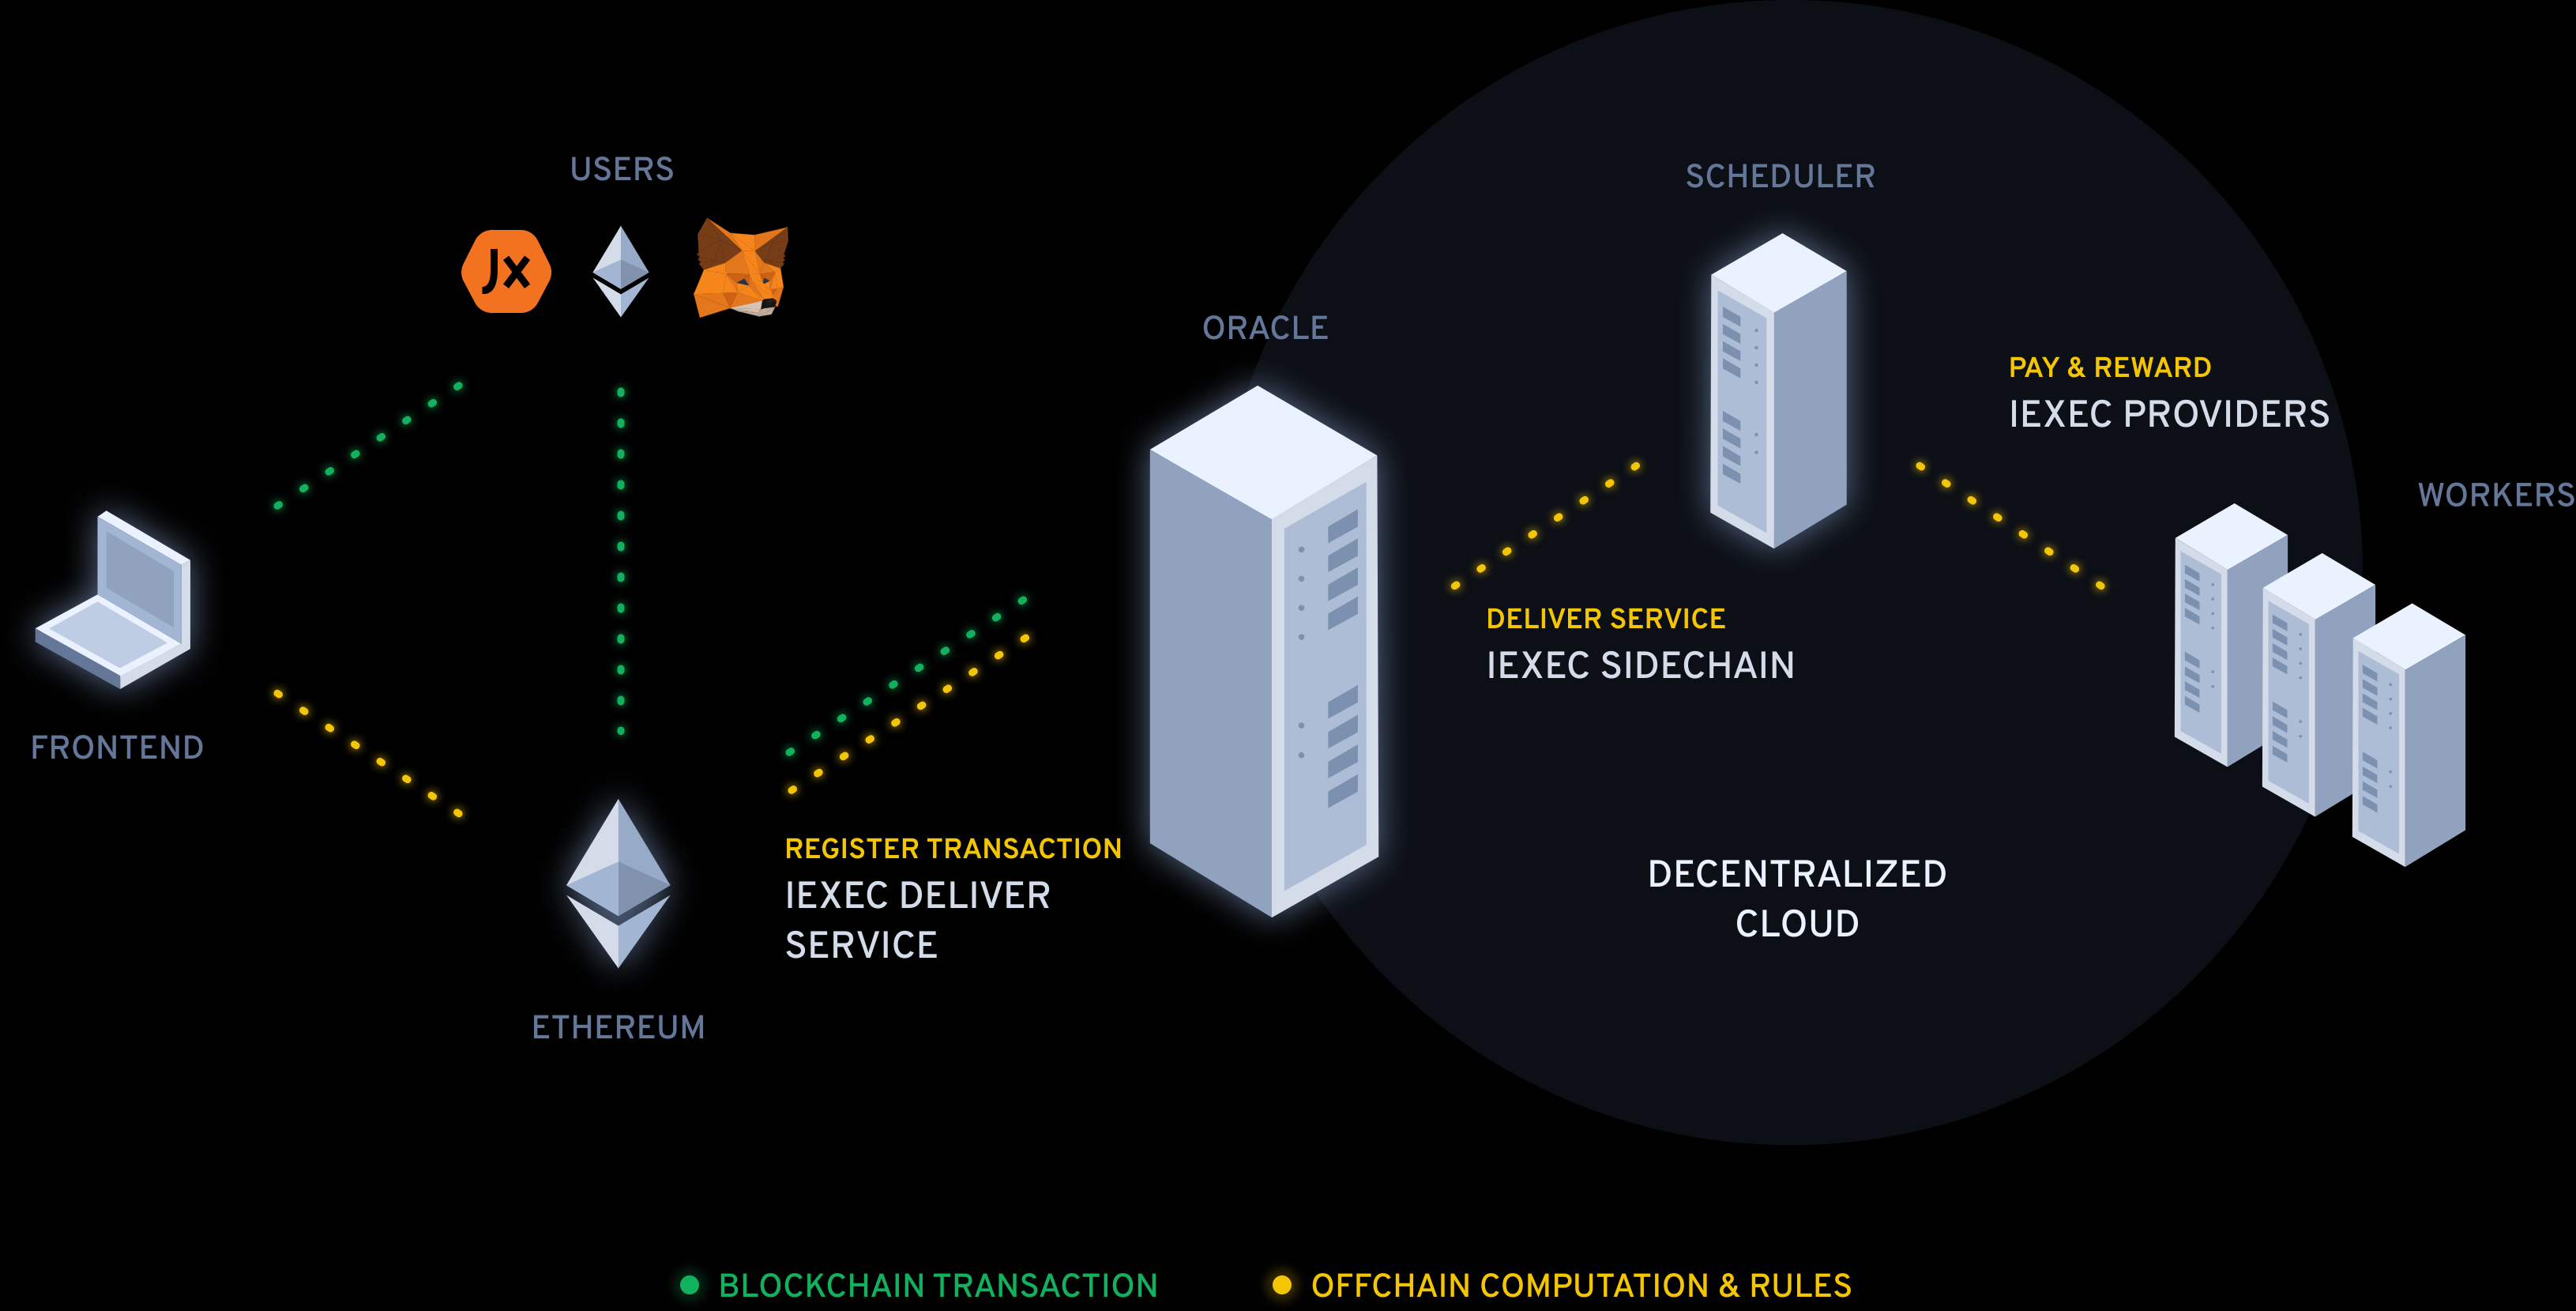
\includegraphics[width=\columnwidth]{4-Requirements/figs/iexec-decentralized-cloud.png}
                \caption{iExec decentralized cloud architecture}
            \end{figure}
        \end{landscape}

        The following figure\cite{iexec-marketplace} presents the iExec ecosystem and highlights the different parts of it
        including the marketplace and the worker pools.

        \begin{figure}[!h]
            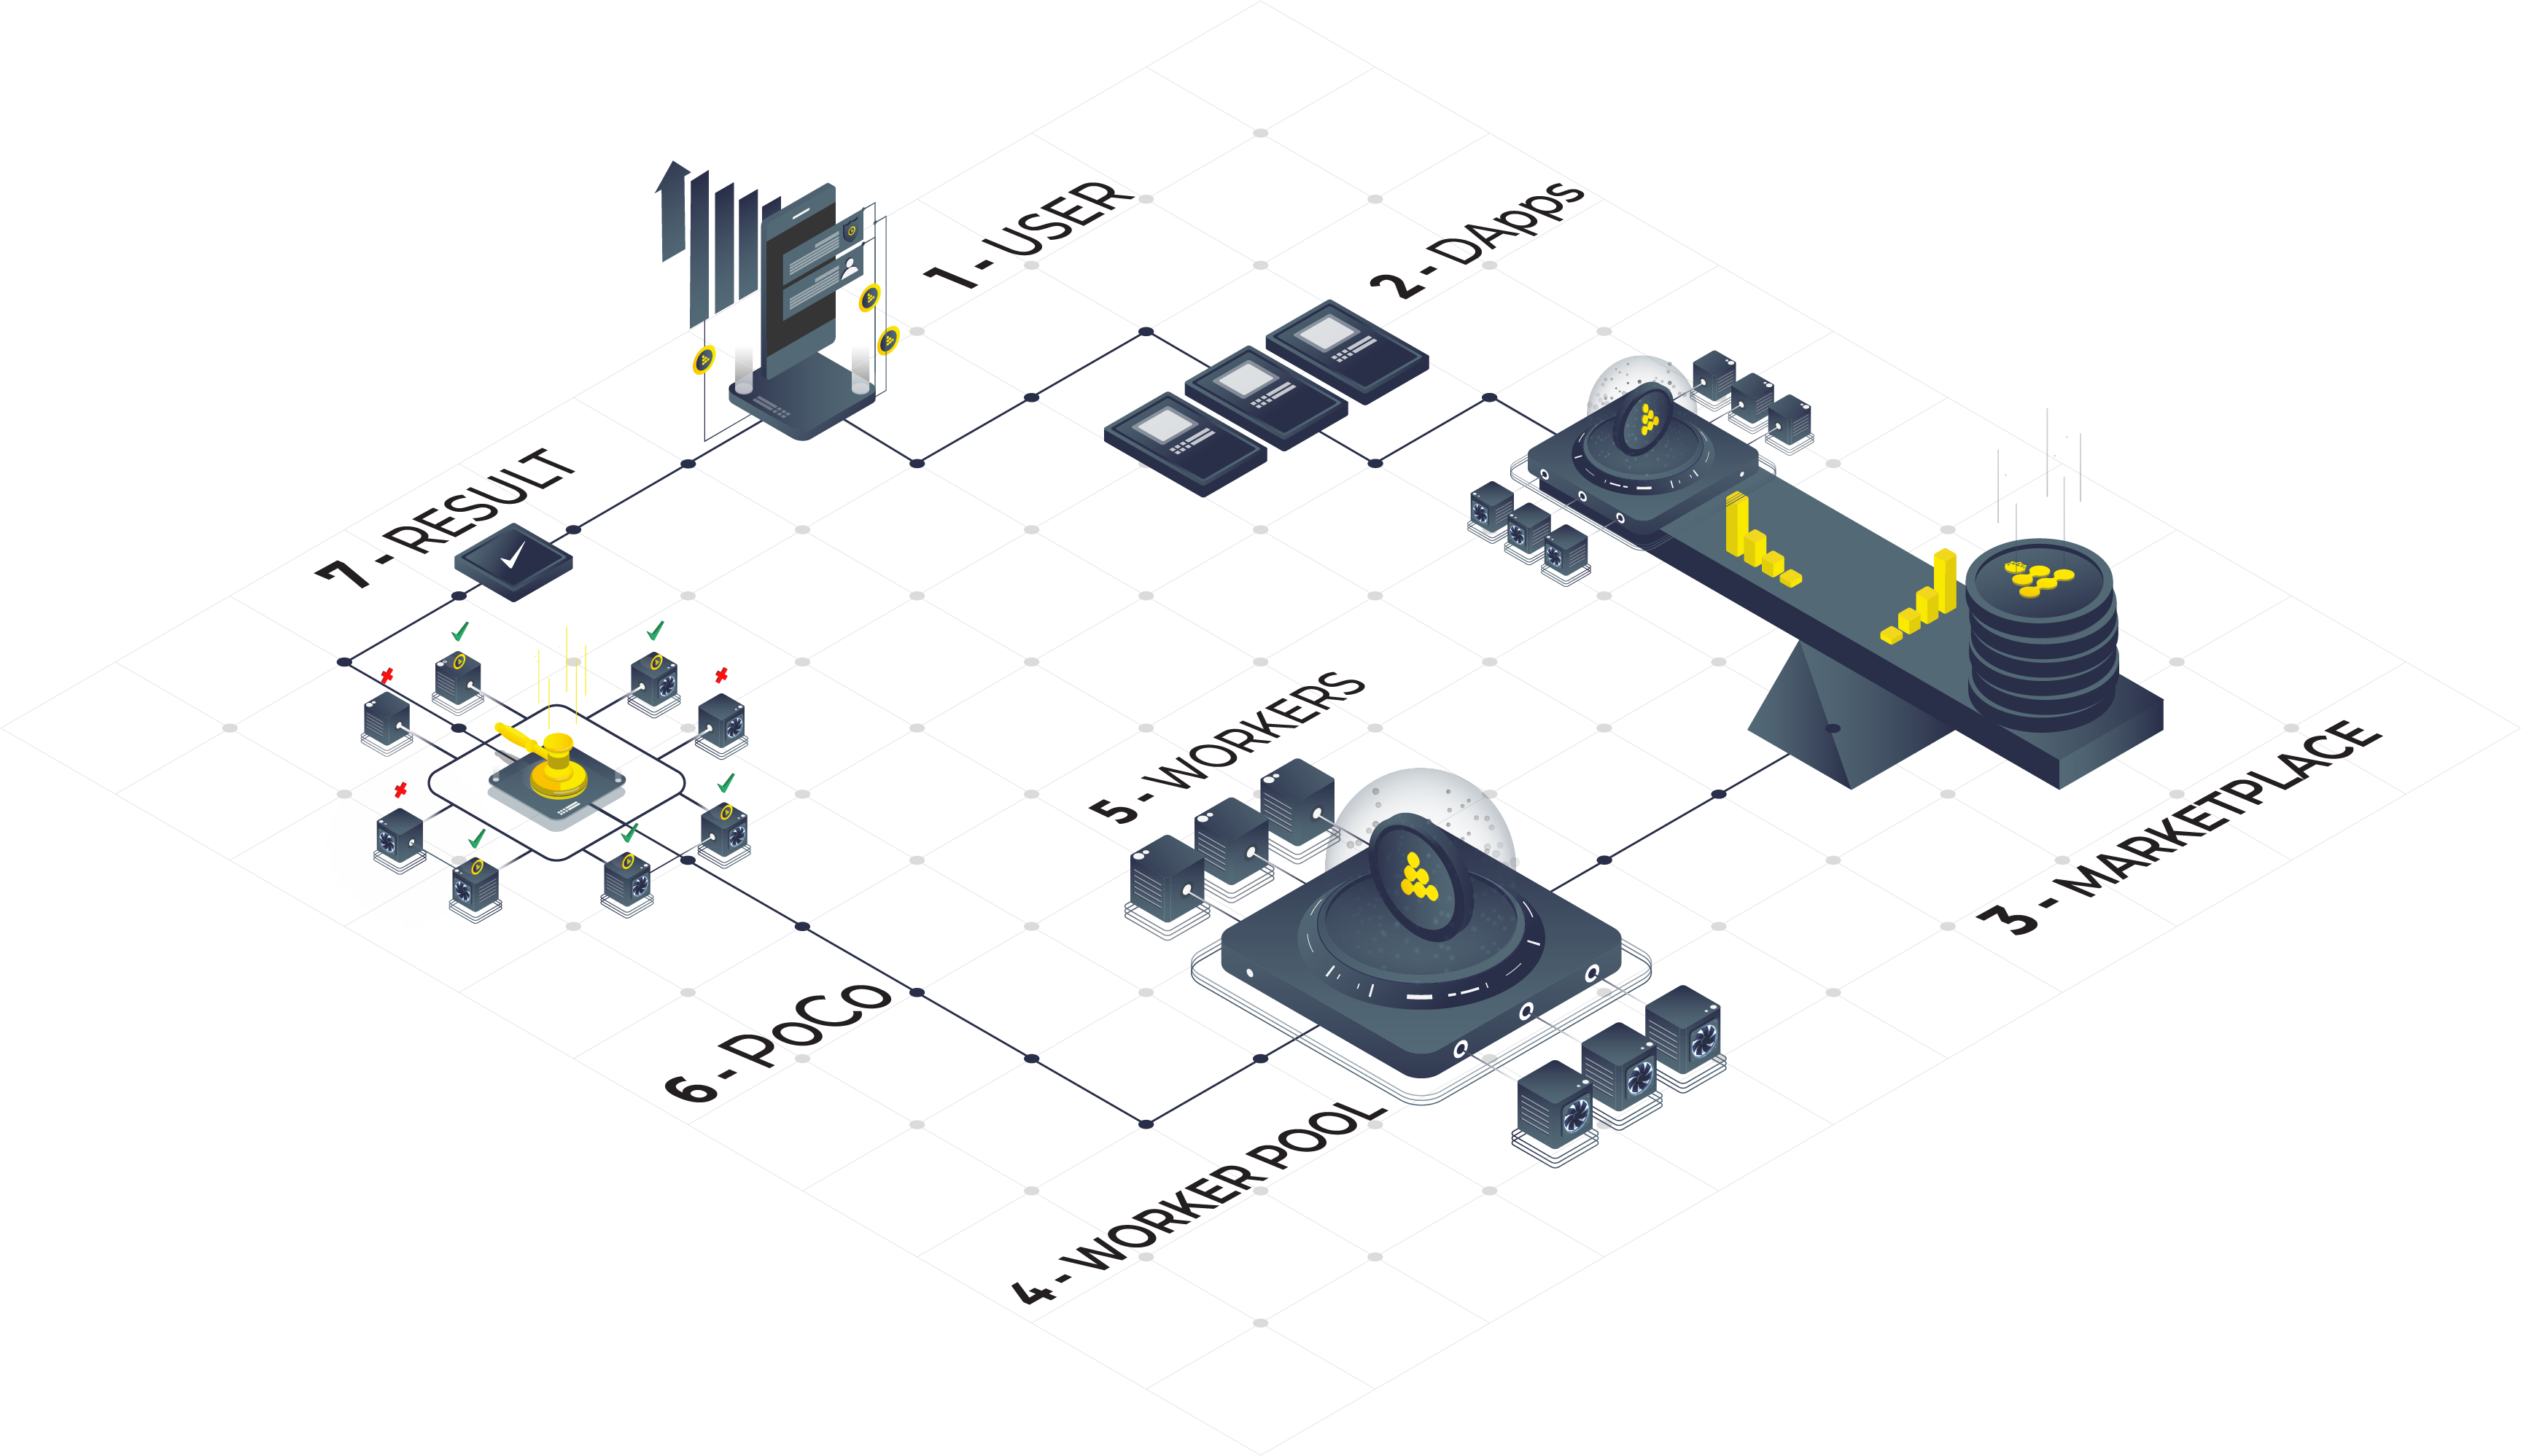
\includegraphics[width=\columnwidth]{4-Requirements/figs/iexec-marketplace.png}
            \caption{iExec marketplace}
        \end{figure}

    \subsection{General Sequence Diagram}
        The worker is one of three components of the global architecture, in addition to the scheduler and the user.
        The user starts the process by issuing and order (sending a job to be executed). The scheduler does the verification
        of the funds for all parts. It checks the accounts of the user and the worker and insures that they have enough RLC,
        delegates the job to the worker, gets the result, runs the PoCo to verify the execution, if no problem occurs it
        finalizes the payment and sends the result back to the user. The worker's mission starts once the job is delegated,
        it downloads the docker image of the application, downloads also the data needed by the execution, executes the task
        and uploads the result back to the scheduler. The worker has always to communicate with the scheduler to update his
        status (alive, working, waiting for work...) and give the scheduler the ability to track the execution process.\newline

        The sequence diagram illustrates the details of all the process:
        
        \begin{figure}[p]
            \vspace*{-2cm}
            \makebox[\linewidth]{
                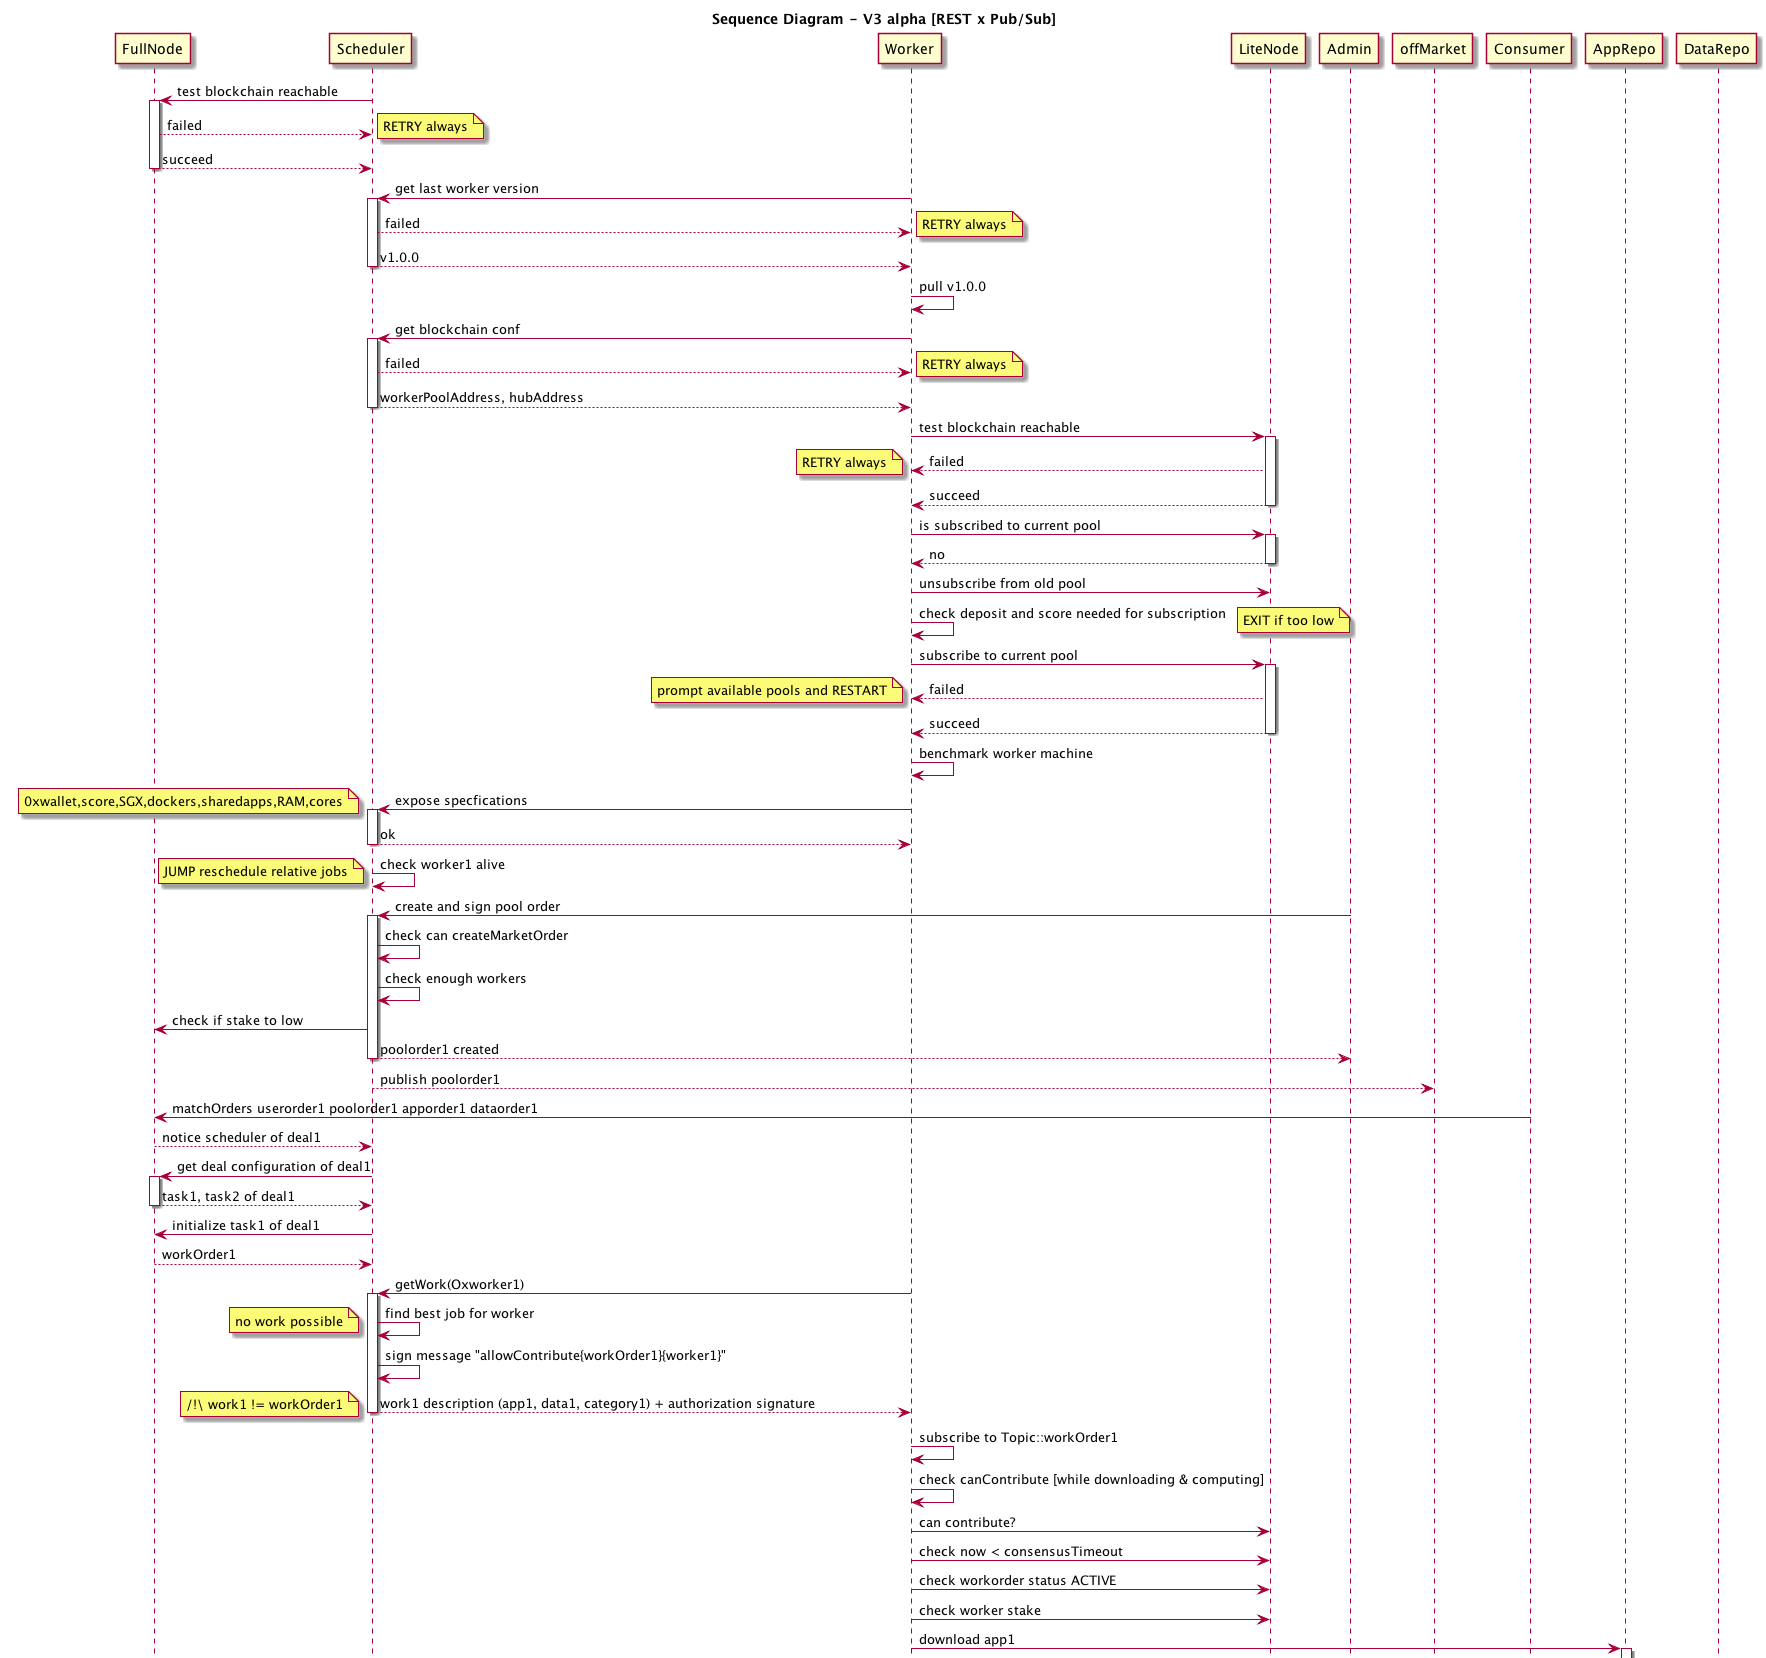
\includegraphics[width=1.3\linewidth]{4-Requirements/figs/iexec-core-sequence-diagram-part-1.png}
            }
            \caption{iExec core sequence diagram - part 1}
        \end{figure}

        \begin{figure}[p]
            \vspace*{-2cm}
            \makebox[\linewidth]{
                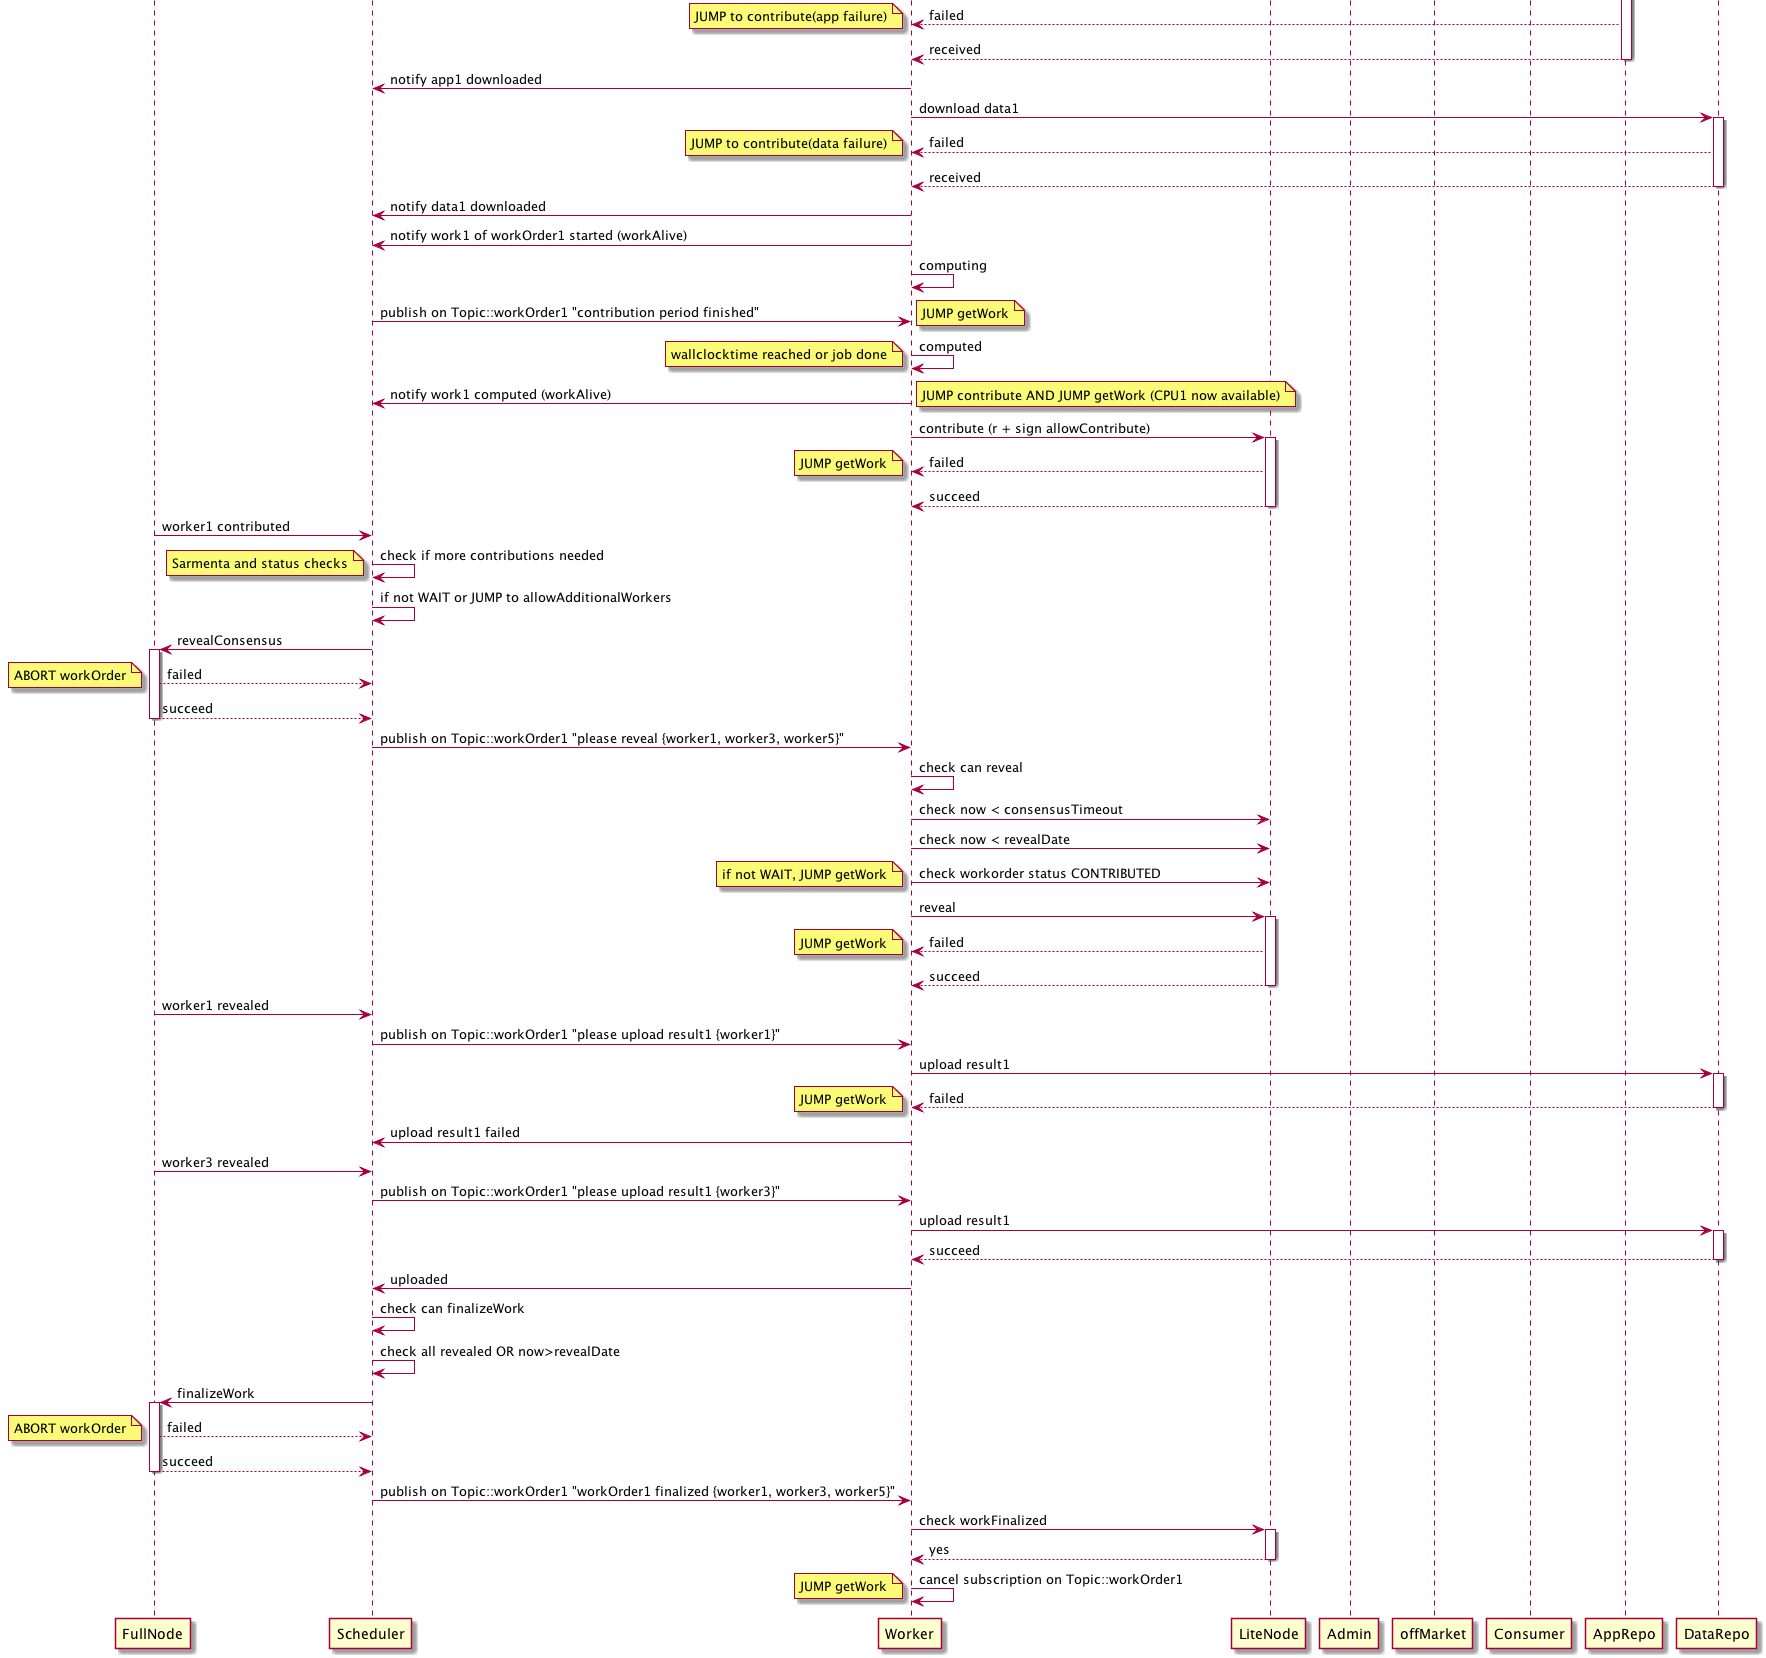
\includegraphics[width=1.3\linewidth]{4-Requirements/figs/iexec-core-sequence-diagram-part-2.png}
            }
            \caption{iExec core sequence diagram - part 2}
        \end{figure}

%******************************** Section 3.3 *********************************%
\section{Requirements}
    \subsection{Functional Requirements}
        The project aims to povide a certain number of functionalities, some of them are absolutely mondatory
        and some others depend on the use case. The main features are listed below.
        \begin{itemize}
            \item \textbf{Execute jobs sent by the middleware:} The worker is a part of iExec's infrastructure, so it
            should execute any type of job sent by XtremWeb middleware, the source of these tasks is blockchain
            dapps that need computation resources. The only constraint that those tasks should repect is the
            specs limitation of the device, Raspberry Pi cards for instance. It's the responsibility of
            the dapps developer and the task sender to deal with this contraint.

            \item \textbf{Ability to prove execution:} The proof-of-contribution\cite{POCO} is the protocole that
            verifies the execution of tasks, so the worker should be able to contribute to the process of the
            verification. In order to achieve that, the worker should have an identity represented by its
            blockchain wallet and its account in the iExec ecosystem.

            \item \textbf{Accomplish the mission of an IoT device:} The worker is always available to execute tasks sent by
            users, but it can also be considered as an IoT device that processes/sends data collected by its sensors.
            For instance, the worker can be a surveillance camera and analyse the video stream to detect motions or
            a weather station that collects informations about the temprature, the humidity, the wind speed ...etc.

            \item \textbf{Ability to manage a cluster of workers:} The project is meant to be applicable on a large number of
            workers, so it is hard to manage them seperatly, that is why it is necessary to have a way to manage them
            easily as a cluster.
        \end{itemize}

    \subsection{Non-Functional Requirements}
        The project emphasizes some extremely important non-functional requirements. Those key specifications should be
        respected in order to maintain the spirit of the project.
        \begin{itemize}
            \item \textbf{Positive energy:} One of the main features of this project is to eliminate the energy cost and
            design a system that is totally green and nature friendly. The worker is powered by solar energy and would
            produce more energy than it consumes. The electricity is saved in a battery to avoid climate's change effects.
            The objectif is to charge the battery with enough electricity for two days.

            \item \textbf{Support ARM architecture:} Who says IoT says ARM\cite{ARM} because this architecture is the
            omnipresent architecture in the IoT ecosystem, so the project has absolutely to support it. The challenge
            would be to build binaries for ARM using non-ARM hardware.
        \end{itemize}

%******************************** Section 3.4 *********************************%
\section{Conclusion}
    After understanding the global architecture of the iExec environment and defining the roles of the different components,
    we identified the functional and non-functional requirements of the project. Those requirements would lead us to the next
    part where we design our system and detail its technical specifications.
    %!TEX root = ../report.tex
%*******************************************************************************
%                              Design & Hardware                               %
%*******************************************************************************


\chapter{Design \& Hardware}

%******************************** Section 4.1 *********************************%
\section{Introduction}
    Once the system requirements are identified, the next step would be to prepare the conceptual representation
    of the project. This part focuses just on the worker, specifying its requirements and going all the way
    from the software and the communication with the scheduler to the hardware specifications.

%******************************** Section 4.2 *********************************%
\section{Design and technical specifications}

    The following diagram presents the interaction between the different components of the worker.
    The connection between the components is guaranteed by the TCP protocol.
    The ports 4321, 4322, 4323 and 4324 should be open in both machines, the worker and the scheduler.
    At the start-up, the worker downloads the CA certificate. This part is mandatory for the program
    to continue working.

    \clearpage

    \begin{figure}[!h]\centering
        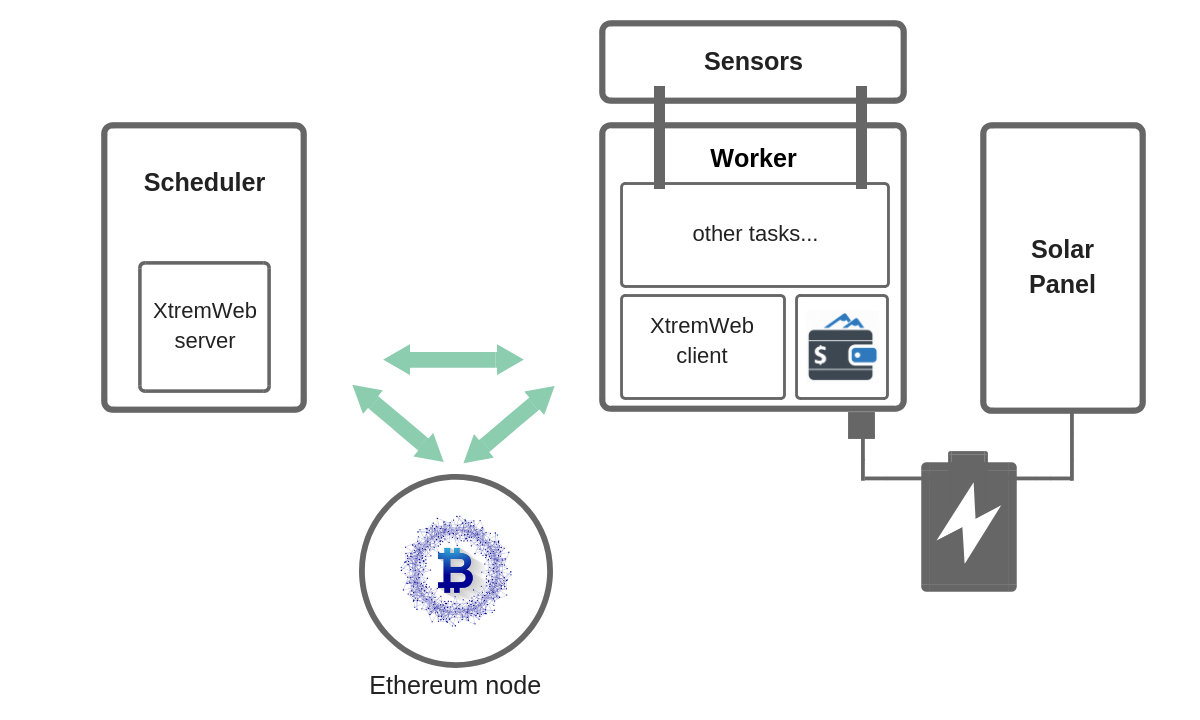
\includegraphics[width=.9\columnwidth]{5-Design/figs/worker-diagram.png}
        \caption{Global overview of the worker design}
    \end{figure}

    We explain in the following subsections the role and requirements of each
    component.

    \subsection{Worker}

        \begin{figure}[!h]\centering
            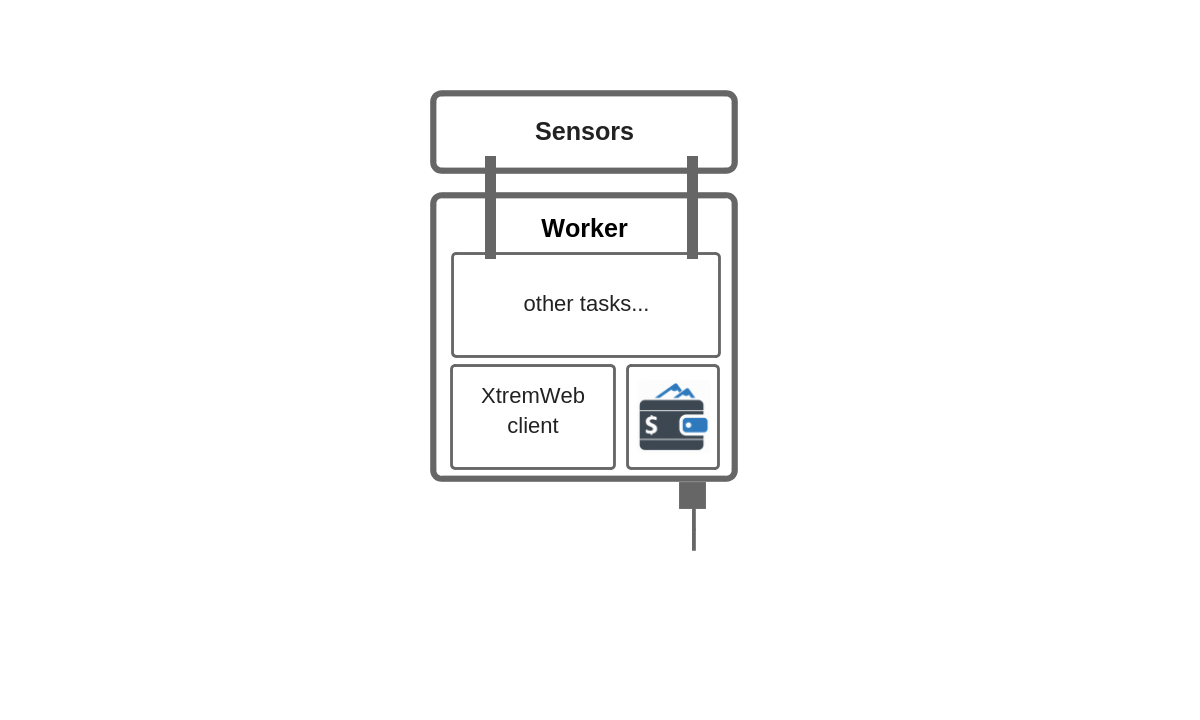
\includegraphics[width=.9\columnwidth]{5-Design/figs/worker.png}
            \caption{The worker internal sortware components}
        \end{figure}

        % \begin{figure}[!h]\centering
        %     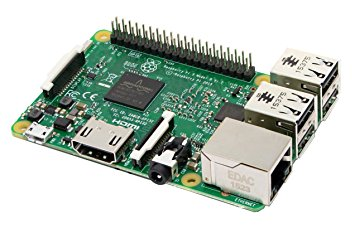
\includegraphics[width=.4\columnwidth]{5-Design/figs/raspberry.jpg}
        %     \caption{The worker internal sortware components}
        % \end{figure}

        The worker runs a docker image of XtremWeb worker. This image has to be optimized for devices with
        limited resources like the Raspberry Pi board.
        XtremWeb does not support ARM architecture natively so this support should be introduced
        to the new version of the middleware. Luckily docker is available for this architecture which simplifies
        the task.

    \subsection{Blockchain}
    
        \begin{figure}[!h]\centering
            \includegraphics[width=.3\columnwidth]{5-Design/figs/blockchain-logo.png}
            \caption{The solar panel}
        \end{figure}

        The blockchain part is represented by the Geth node where we deploy the iExec smart contracts.
        The worker should take care of the necessary blokchain configuration for the proper functioning
        of the system, so it should provide a wallet with sufficient funds (in RLC). The scheduler locks
        an amount of RLC when an execution is starting, so the worker should have the minimum amount
        required by the operation. If these requirements are not satisfied the program will crash.

    \subsection{Use case diagram}
        Use case diagram describes the functionality provided by a system in terms of actors, their
        goals represented as use cases, and any dependencies among those use cases.
        It is therefore to have an external view of the functioning of the system, which on the one hand
        defines the behavior of the system in its environment and on the other hand to identify the needs
        and objectives expected of the actors. At this stage we're going to focus on the worker as our
        system. \newline
        At first we start by introducing the interacting actors, then we present a description about
        functionalities provided. \newline \newline
        \textit{Actors: }
        An actor represents a role played by an external entity that directly interacts with the system
        being studied. Our actors are:
        \begin{itemize}
            \item \textbf{The scheduler: }
            it sends jobs to the worker, waits for the execution to finish, verifies the results and does
            the payment transactions.
            \item \textbf{The external service: }
            This actor does not have effect on the system (worker). It receives the data sent by the worker.
            \item \textbf{The solar panel: }
            It provides the necessary energy for the worker.
        \end{itemize}
        \textit{Use cases: }
        A use case represents a set of action sequences that are performed by the system and that produce
        an observable result of interest for a particular actor.

        \begin{itemize}
            \item \textbf{Scheduler}
                \begin{itemize}
                    \item Delegate jobs: the scheduler sends the description of received tasks to the worker
                    to execute it.
                    \item Get the result of execution: after the execution the worker sends the result back
                    to the scheduler.
                    \item Pay execution: the scheduler sends the reward to the worker.
                \end{itemize}
            
            \item \textbf{External service}
                \begin{itemize}
                    \item Subscribe to data stream: The service subscribes to receive the data.
                    \item Receive processed data stream: The service receives the collected data sent by the
                    worker.
                \end{itemize}
            
            \item \textbf{Solar panel}
                \begin{itemize}
                    \item Implement the energy produced: the panel supplies the worker with the necessary energy.
                \end{itemize}
        \end{itemize}


        \begin{figure}[!h]\centering
            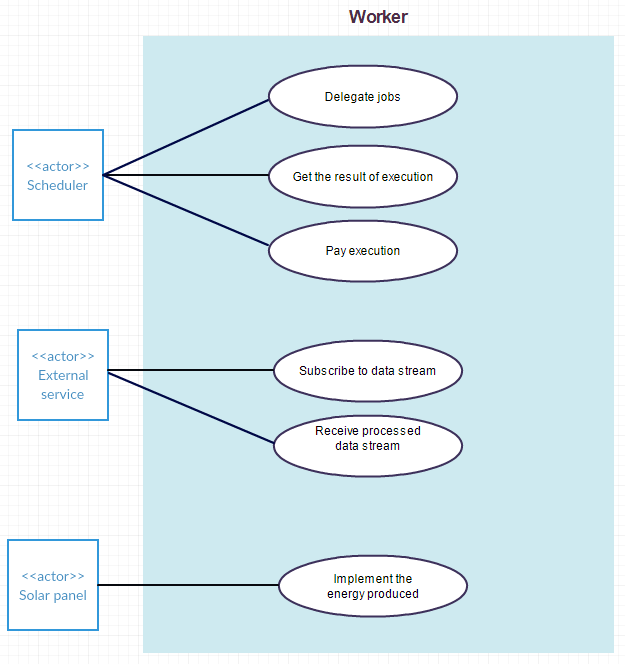
\includegraphics[width=\columnwidth]{5-Design/figs/use-case-diagram.png}
            \caption{Worker use case diagram}
        \end{figure}

        \clearpage

%******************************** Section 4.3 *********************************%
\section{Hardware}

    \subsection{Solar Panel}

        \begin{figure}[!h]\centering
            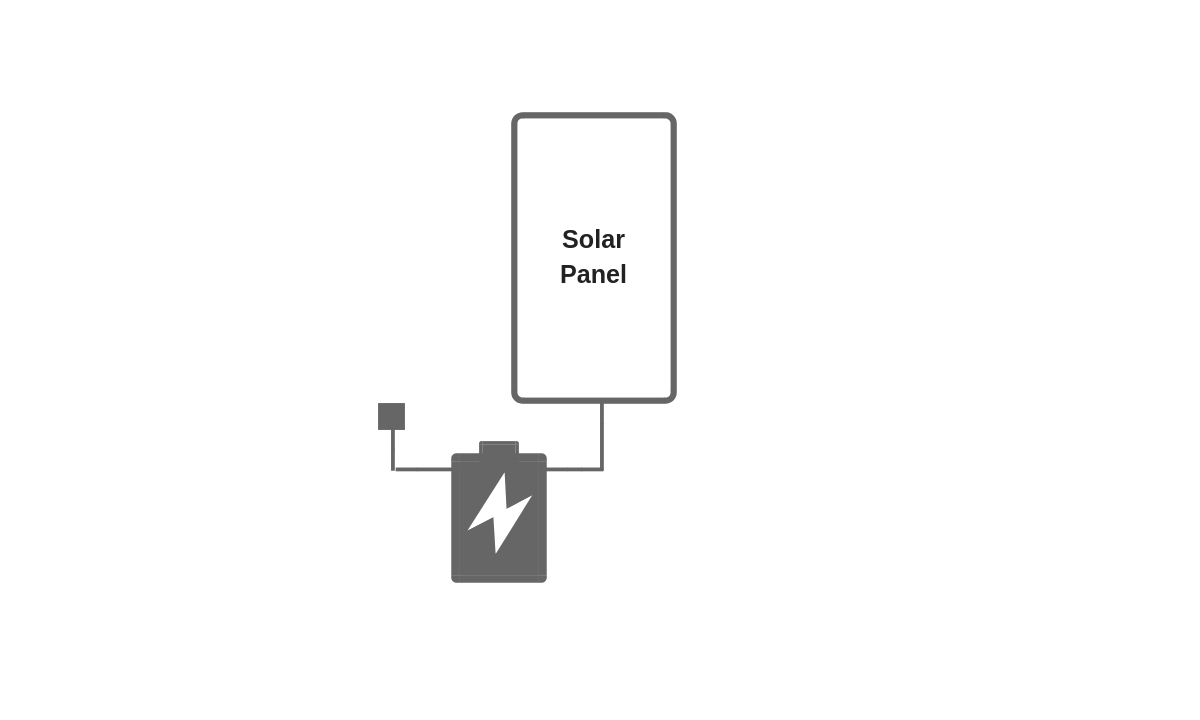
\includegraphics[width=.6\columnwidth]{5-Design/figs/solar-panel.png}
            \caption{The solar panel}
        \end{figure}

        A Photovoltaic solar panels is used to power the worker. It absorbs sunlight as a source of energy to
        generate electricity and charge the battery. In this case we use a panel with high conversion
        efficiency: 60 watt SUNPOWER mono-crystalline with conversion efficiency up to 25\% which is much
        higher than common solar panel charger (15\%).

        Reference of the chosen panel: SUAOKI 60W Portable Sunpower Mono-crystalline Solar Panel with DC 18V and USB
        5V Output Charger.\newline
        Output: up to 60W - USB: 18v/3.4A, DC: 5v/2.5A.

        \begin{figure}[!h]\centering
            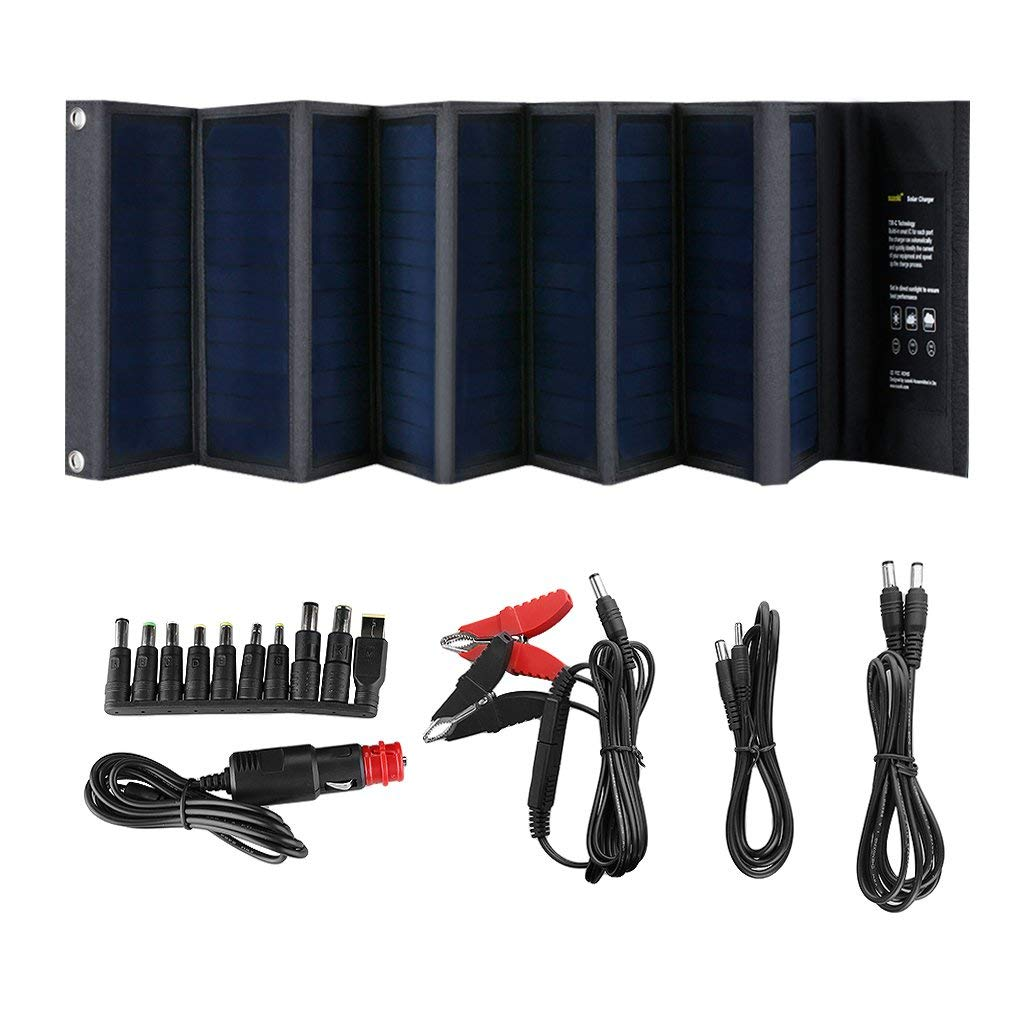
\includegraphics[width=.4\columnwidth]{5-Design/figs/panel.jpg}
            \caption{SUNPOWER solar panel}
        \end{figure}

        This panel should be able to charge the battery in merely 8 hours during a sunny day. The Raspberry
        Pi board consumes 1A for a maximum utilization of the CPU and some plugged sensors. For a battery
        capacity of 50000mA, the worker can stay up for 24 hours for a full battery without any source of
        solar light.

    \subsection{Battery}

        \begin{figure}[!h]\centering
            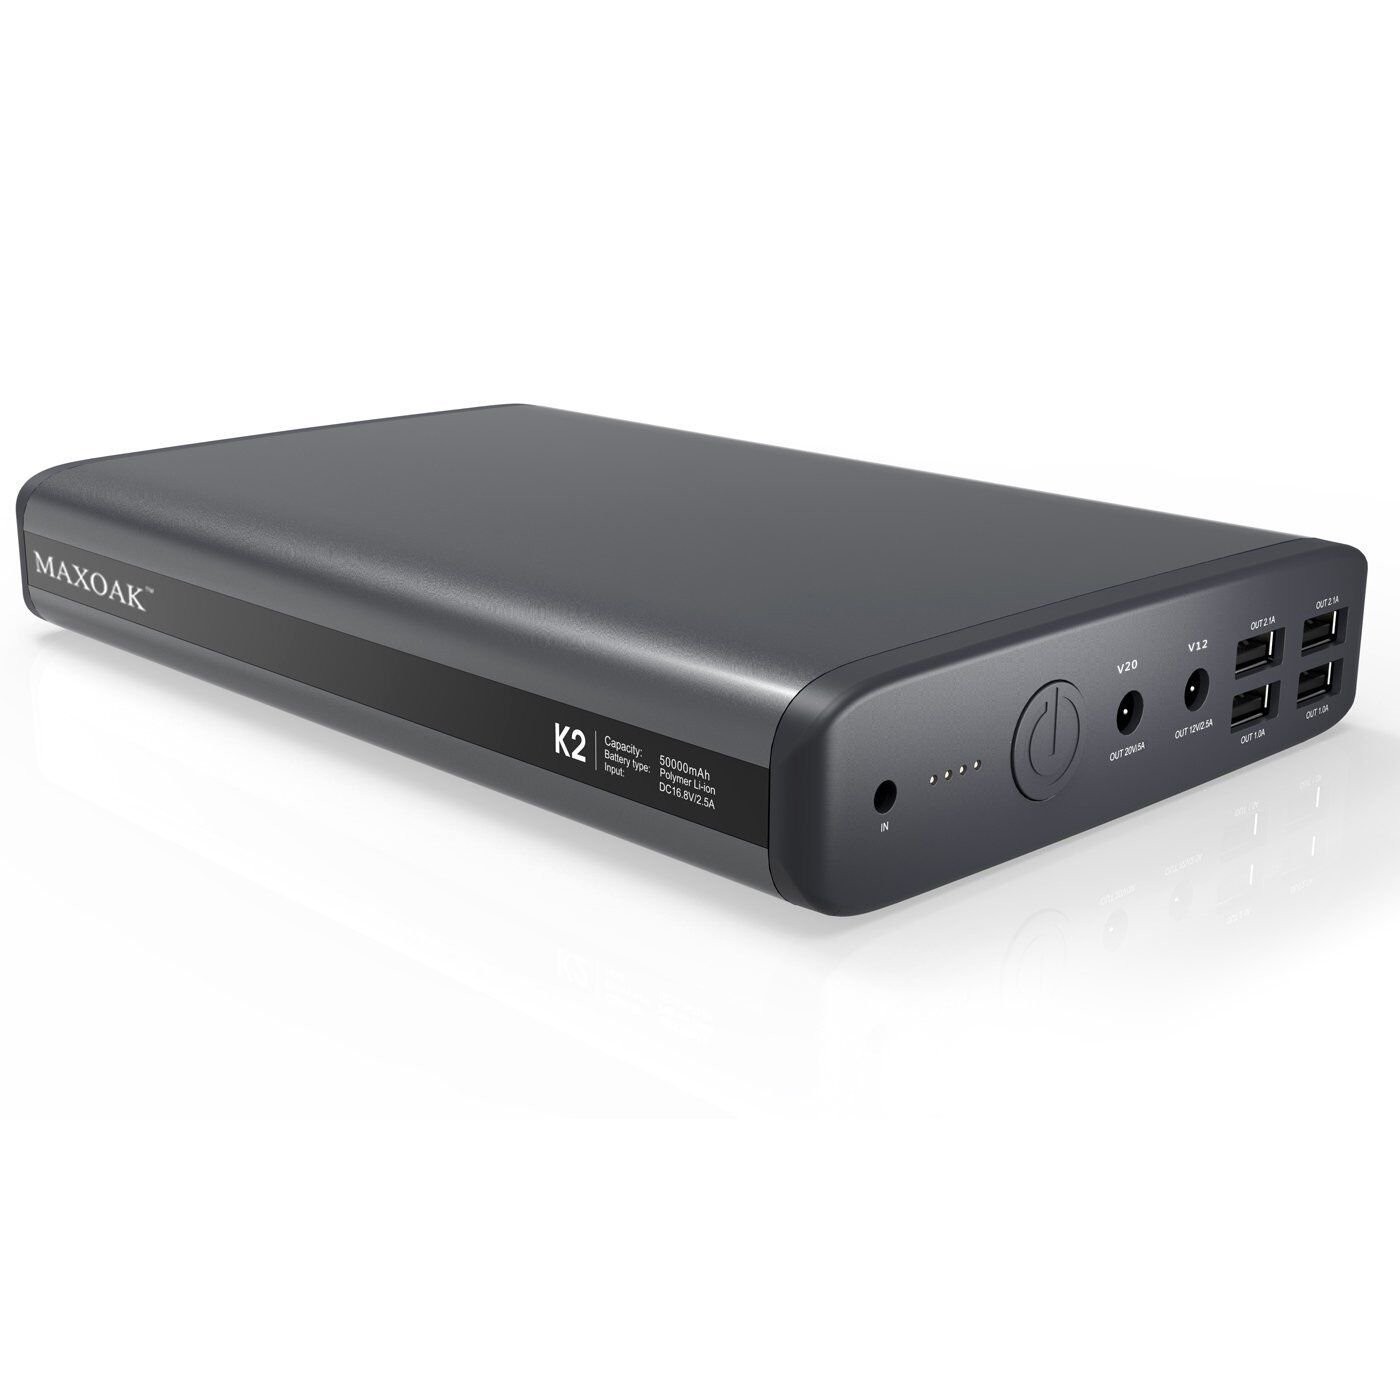
\includegraphics[width=.3\columnwidth]{5-Design/figs/battery.jpg}
            \caption{50000 mA Battery}
        \end{figure}

        We suppose that the battery should be able to store electricity for, at least, two days. With a
        consumption of maximum 24A/day, the battery should store 50A. It should also contain a 5V output
        to power the worker with the right intensity.

        Reference of the chosen battery: MAXOAK 50000mAh 5/12/20v Portable Charger External Battery Power Bank.

    \subsection{Sensors}
        The worker uses different sensors to interact with the outside world. We can imagine multiple systems
        with a lot of use cases. We will take as example two use cases:

        \underline{Surveillance camera:} the worker has an 8 megapixel native resolution sensor-capable of 3280 x 2464
        pixel static images camera to achieve the mission of a surveillance system that streams video and detects motions.

        \begin{figure}[!h]\centering
            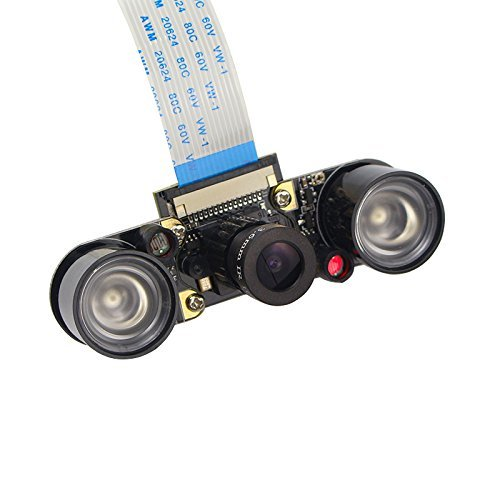
\includegraphics[width=.2\columnwidth]{5-Design/figs/camera.jpg}
            \caption{Raspberry Pi camera}
        \end{figure}


        \underline{Weather station:} in this case the worker uses a humidity, pressure, temprature and
        orientation senors to build a weather station. It collects weather data and applies some
        processing on it before sending it to a weather forcast service. The data processing can be done
        with an iExec dapp locally on the worker and this model has many advantges such as pushing the
        processing to the edge of the network to reduce latency caused by data transfer and enhance data
        privacy because it is not leaving the device.

        \begin{figure}[!h]\centering
            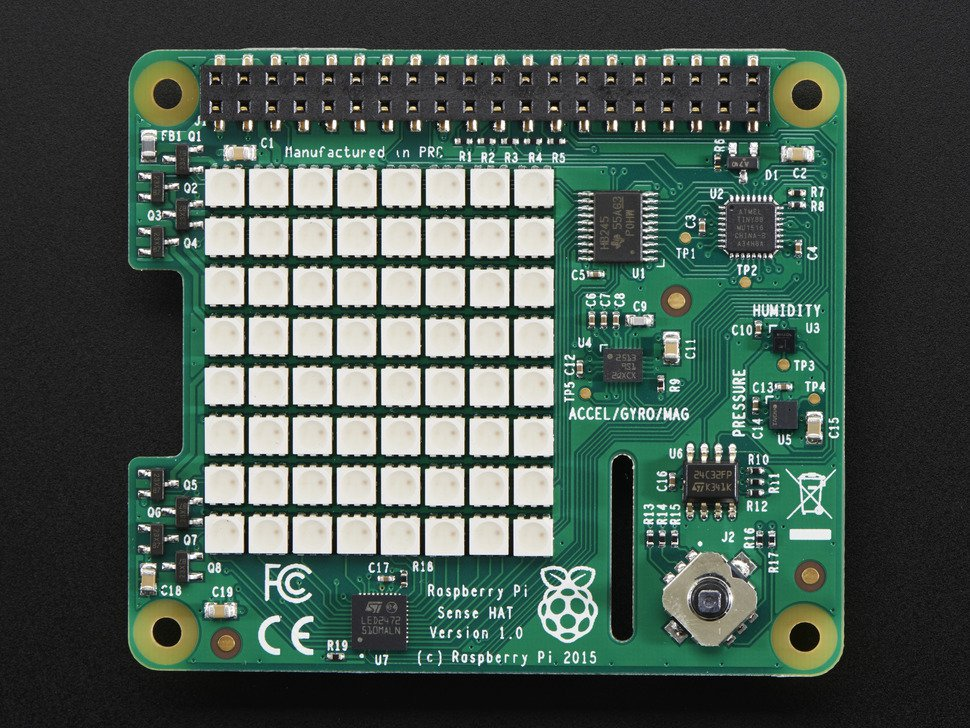
\includegraphics[width=.3\columnwidth]{5-Design/figs/sense-hat.jpg}
            \caption{Raspberry Pi Sense HAT}
        \end{figure}

%******************************** Section 4.4 *********************************%
\section{Conclusion}
    In this chapter, we worked on the first place on designing the worker taking in consideration the resources
    limitation of the worker board. In the second section, we worked on choosing the hardware that suits
    the requirements, therefore we pass to the implementation part to shape our design.
    %!TEX root = ../thesis.tex
%*******************************************************************************
%                            Implementation                                  %
%*******************************************************************************


\chapter{Implementation}

% **************************** Define Graphics Path **************************
% \ifpdf
%     \graphicspath{{Chapter3/Figs/Raster/}{Chapter3/Figs/PDF/}{Chapter3/Figs/}}
% \else
%     \graphicspath{{Chapter3/Figs/Vector/}{Chapter3/Figs/}}
% \fi


\section{Introduction}
- intro

\section{Work environment}
    \subsection{Hardware environment}
        \subsection{Electronic Card: Raspberry Pi}
        \subsection{Solar Panel}
        \subsection{Battery}
        \subsection{Witty Pi}
    \subsection{Software environment}
        \subsection{Development Technologies}
        \subsection{Documentation}

\section{Illustration}

\section{Conclusion}


    %!TEX root = ../thesis.tex
%*******************************************************************************
%                    General Conclusion And Perspectives                       %
%*******************************************************************************


\chapter*{General Conclusion And Perspectives} \addcontentsline{toc} {chapter} {General Conclusion And Perspectives}

% **************************** Define Graphics Path **************************
\ifpdf
    \graphicspath{{Chapter3/Figs/Raster/}{Chapter3/Figs/PDF/}{Chapter3/Figs/}}
\else
    \graphicspath{{Chapter3/Figs/Vector/}{Chapter3/Figs/}}
\fi


    
    
    % ********************************** Back Matter *******************************
    % Backmatter should be commented out, if you are using appendices after References
    % \backmatter
    
    
    % ********************************** Bibliography ******************************
    \begin{spacing}{0.9}
    
    % To use the conventional natbib style referencing
    % Bibliography style previews: http://nodonn.tipido.net/bibstyle.php
    % Reference styles: http://sites.stat.psu.edu/~surajit/present/bib.htm
    
    % \bibliographystyle{apalike}
    \bibliographystyle{unsrt} % Use for unsorted references  
    %\bibliographystyle{plainnat} % use this to have URLs listed in References
    \cleardoublepage
    \bibliography{8-References/references} % Path to your References.bib file
    
    % ********************************** Appendices ******************************
    % \bibliography{9-Appendices/appendix}
    
    % ********************************** Summaries ******************************
    \bibliography{10.0-English-summary/summary}
    \bibliography{10.1-Frensh-summary/summary}
    \bibliography{10.2-Arabic-summary/summary}

    
    % If you would like to use BibLaTeX for your references, pass `custombib' as
    % an option in the document class. The location of 'reference.bib' should be
    % specified in the preamble.tex file in the custombib section.
    % Comment out the lines related to natbib above and uncomment the following line.
    
    % \printbibliography[heading=bibintoc, title={References}]

    \end{spacing}
    

    % ********************************** Appendices ********************************
    
    % \begin{appendices} % Using appendices environment for more functionality
    
    % %!TEX root = ../thesis.tex
% ******************************* Thesis Appendix A ****************************
\chapter{How to install \LaTeX} 

\section*{Windows OS}

\subsection*{TeXLive package - full version}
\begin{enumerate}
\item	Download the TeXLive ISO (2.2GB) from\\
\href{https://www.tug.org/texlive/}{https://www.tug.org/texlive/}
\item	Download WinCDEmu (if you don't have a virtual drive) from \\
\href{http://wincdemu.sysprogs.org/download/}
{http://wincdemu.sysprogs.org/download/}
\item	To install Windows CD Emulator follow the instructions at\\
\href{http://wincdemu.sysprogs.org/tutorials/install/}
{http://wincdemu.sysprogs.org/tutorials/install/}
\item	Right click the iso and mount it using the WinCDEmu as shown in \\
\href{http://wincdemu.sysprogs.org/tutorials/mount/}{
http://wincdemu.sysprogs.org/tutorials/mount/}
\item	Open your virtual drive and run setup.pl
\end{enumerate}

or

\subsection*{Basic MikTeX - \TeX~ distribution}
\begin{enumerate}
\item	Download Basic-MiK\TeX (32bit or 64bit) from\\
\href{http://miktex.org/download}{http://miktex.org/download}
\item	Run the installer 
\item	To add a new package go to Start >> All Programs >> MikTex >> Maintenance (Admin) and choose Package Manager
\item	Select or search for packages to install
\end{enumerate}

\subsection*{TexStudio - \TeX~ editor}
\begin{enumerate}
\item	Download TexStudio from\\
\href{http://texstudio.sourceforge.net/\#downloads}
{http://texstudio.sourceforge.net/\#downloads} 
\item	Run the installer
\end{enumerate}

\section*{Mac OS X}
\subsection*{MacTeX - \TeX~ distribution}
\begin{enumerate}
\item	Download the file from\\
\href{https://www.tug.org/mactex/}{https://www.tug.org/mactex/}
\item	Extract and double click to run the installer. It does the entire configuration, sit back and relax.
\end{enumerate}

\subsection*{TexStudio - \TeX~ editor}
\begin{enumerate}
\item	Download TexStudio from\\
\href{http://texstudio.sourceforge.net/\#downloads}
{http://texstudio.sourceforge.net/\#downloads} 
\item	Extract and Start
\end{enumerate}


\section*{Unix/Linux}
\subsection*{TeXLive - \TeX~ distribution}
\subsubsection*{Getting the distribution:}
\begin{enumerate}
\item	TexLive can be downloaded from\\
\href{http://www.tug.org/texlive/acquire-netinstall.html}
{http://www.tug.org/texlive/acquire-netinstall.html}.
\item	TexLive is provided by most operating system you can use (rpm,apt-get or yum) to get TexLive distributions
\end{enumerate}

\subsubsection*{Installation}
\begin{enumerate}
\item	Mount the ISO file in the mnt directory
\begin{verbatim}
mount -t iso9660 -o ro,loop,noauto /your/texlive####.iso /mnt
\end{verbatim}

\item	Install wget on your OS (use rpm, apt-get or yum install)
\item	Run the installer script install-tl.
\begin{verbatim}
	cd /your/download/directory
	./install-tl
\end{verbatim}
\item	Enter command `i' for installation

\item	Post-Installation configuration:\\
\href{http://www.tug.org/texlive/doc/texlive-en/texlive-en.html\#x1-320003.4.1}
{http://www.tug.org/texlive/doc/texlive-en/texlive-en.html\#x1-320003.4.1} 
\item	Set the path for the directory of TexLive binaries in your .bashrc file
\end{enumerate}

\subsubsection*{For 32bit OS}
For Bourne-compatible shells such as bash, and using Intel x86 GNU/Linux and a default directory setup as an example, the file to edit might be \begin{verbatim}
edit $~/.bashrc file and add following lines
PATH=/usr/local/texlive/2011/bin/i386-linux:$PATH; 
export PATH 
MANPATH=/usr/local/texlive/2011/texmf/doc/man:$MANPATH;
export MANPATH 
INFOPATH=/usr/local/texlive/2011/texmf/doc/info:$INFOPATH;
export INFOPATH
\end{verbatim}
\subsubsection*{For 64bit OS}
\begin{verbatim}
edit $~/.bashrc file and add following lines
PATH=/usr/local/texlive/2011/bin/x86_64-linux:$PATH;
export PATH 
MANPATH=/usr/local/texlive/2011/texmf/doc/man:$MANPATH;
export MANPATH 
INFOPATH=/usr/local/texlive/2011/texmf/doc/info:$INFOPATH;
export INFOPATH

\end{verbatim}



%\subsection{Installing directly using Linux packages} 
\subsubsection*{Fedora/RedHat/CentOS:}
\begin{verbatim} 
sudo yum install texlive 
sudo yum install psutils 
\end{verbatim}


\subsubsection*{SUSE:}
\begin{verbatim}
sudo zypper install texlive
\end{verbatim}


\subsubsection*{Debian/Ubuntu:}
\begin{verbatim} 
sudo apt-get install texlive texlive-latex-extra 
sudo apt-get install psutils
\end{verbatim}

    % %!TEX root = ../thesis.tex
% ******************************* Thesis Appendix B ********************************

\chapter{Installing the CUED class file}

\LaTeX.cls files can be accessed system-wide when they are placed in the
<texmf>/tex/latex directory, where <texmf> is the root directory of the user’s \TeX installation. On systems that have a local texmf tree (<texmflocal>), which
may be named ``texmf-local'' or ``localtexmf'', it may be advisable to install packages in <texmflocal>, rather than <texmf> as the contents of the former, unlike that of the latter, are preserved after the \LaTeX system is reinstalled and/or upgraded.

It is recommended that the user create a subdirectory <texmf>/tex/latex/CUED for all CUED related \LaTeX class and package files. On some \LaTeX systems, the directory look-up tables will need to be refreshed after making additions or deletions to the system files. For \TeX Live systems this is accomplished via executing ``texhash'' as root. MIK\TeX users can run ``initexmf -u'' to accomplish the same thing.

Users not willing or able to install the files system-wide can install them in their personal directories, but will then have to provide the path (full or relative) in addition to the filename when referring to them in \LaTeX.
    
    % \end{appendices}
    
    % *************************************** Index ********************************
    \printthesisindex % If index is present
    
    \end{document}
    